\documentclass[sn-mathphys,Numbered]{sn-jnl}% Math and Physical Sciences Reference Style
%\documentclass[sn-mathphys,Numbered,draft]{sn-jnl}% Math and Physical Sciences Reference Style

%%\documentclass[sn-nature]{sn-jnl}% Style for submissions to Nature Portfolio journals
%%\documentclass[sn-basic]{sn-jnl}% Basic Springer Nature Reference Style/Chemistry Reference Style
%%\documentclass[sn-aps]{sn-jnl}% American Physical Society (APS) Reference Style
%%\documentclass[sn-vancouver,Numbered]{sn-jnl}% Vancouver Reference Style
%%\documentclass[sn-apa]{sn-jnl}% APA Reference Style 
%%\documentclass[sn-chicago]{sn-jnl}% Chicago-based Humanities Reference Style
%%\documentclass[default]{sn-jnl}% Default
%%\documentclass[default,iicol]{sn-jnl}% Default with double column layout

%%%% Standard Packages
%%<additional latex packages, if required can be included here>

\setlength{\parskip}{\baselineskip}

\usepackage{graphicx}%
\usepackage{amsmath,amssymb,amsfonts,bm}%
\usepackage{multirow}
\usepackage{amsthm}%
%\usepackage{subcaption}
\usepackage{mathrsfs}%
\usepackage[title]{appendix}%
\usepackage{xcolor}%
\usepackage{textcomp}%
\usepackage{manyfoot}%
\usepackage{booktabs}%
%\usepackage{algorithm}%
%\usepackage{algorithmicx}%
\usepackage{algpseudocode}%
\usepackage{listings}%
\usepackage{bigints}
\usepackage{outlines}
\usepackage{geometry}
\usepackage{subfigure}
\usepackage{siunitx}
\usepackage{float}
\usepackage{comment}

\geometry
{
a4paper,         % or letterpaper
textwidth=15cm,  % llncs has 12.2cm
textheight=24cm, % llncs has 19.3cm
% heightrounded,   % integer number of lines
% hratio=1:1,      % horizontally centered
% vratio=2:3,      % not vertically centered
}
\setlength{\tabcolsep}{0.5cm}
\usepackage[onehalfspacing]{setspace}
% \usepackage{lineno}
% \linenumbers
%%%%

\usepackage[utf8]{inputenc}
\usepackage{graphicx}
\usepackage[ruled,vlined]{algorithm2e}
\usepackage{amsmath}
%\usepackage{movie15} %to allow movie embedding
\usepackage[section]{placeins}
\usepackage{enumitem}
\usepackage{color,soul}
\usepackage{xfrac}

%% New math commands
\newcommand{\s}[1]{\overset{*}{#1}}
\newcommand{\RM}{\bm{\Lambda}}
\newcommand{\RMI}{\bm{\Lambda}_0}
\newcommand{\RMT}{\bm{\Lambda}_t}
\newcommand{\RV}{\bm{\psi}}
\newcommand{\magRV}{\psi}
\newcommand{\RMTS}{\s{\bm{\Lambda}}_t}
\newcommand{\bb}{\boldsymbol}
\usepackage{nicefrac}
%\usepackage{tikz}
%\usepackage{tikz-3dplot}
\usepackage{mathtools}

%% For contact
\newcommand{\rbar}{\bar{\bm{r}}}
\newcommand{\xibar}{\bar{\xi}}
%\newcommand{\magRV}{\bbit{\psi}}
\newcommand{\diag}{\rm diag}

\begin{document}

\title[Article Title]{A monolithic cell-centred finite volume approach for fluid-solid interaction}

\author*[1]{\fnm{Philip} \sur{Cardiff}}\email{philip.cardiff@ucd.ie}
%\author*[1,2,3]{\fnm{Philip} \sur{Cardiff}}\email{philip.cardiff@ucd.ie}
%\author[1,2,3]{\fnm{Dylan} \sur{Armfield}}
%%\author[5]{\fnm{Hiroaki} \sur{Nishikawa}}
%\author[4]{\fnm{\v{Z}eljko} \sur{Tukovi\'{c}}}
%\author[4]{\fnm{Ivan} \sur{Batisti\'{c}}}

\affil*[1]{\orgdiv{School of Mechanical and Materials Engineering}, \orgname{University College Dublin}, \orgaddress{\country{Ireland}}}
%\affil[2]{\orgdiv{UCD Centre for Mechanics}, \orgname{University College Dublin}, \orgaddress{\country{Ireland}}}
%\affil[3]{\orgdiv{I-Form Centre}, \orgname{University College Dublin}, \orgaddress{\country{Ireland}}}
%\affil[4]{\orgdiv{Faculty of Mechanical Engineering and Naval Architecture}, \orgname{University of Zagreb}, \orgaddress{\country{Croatia}}}
%\affil[5]{\orgname{National Institute of Aerospace}, \orgaddress{\country{Hampton, VA 23666, USA}}}



\abstract
{
WIP
}



\keywords{Fluid-solid interaction, Monolithic, Jacobian-free Newton-Krylov, Finite volume method, solids4foam, OpenFOAM}

\maketitle


%%%%%%%%%%%%%%%%%%%%%%%%%%%%%%%%%%%%%%%%%%%%%%%%%%%%%%%%%%%%%
\section{Introduction}\label{sec:intro}
%%%%%%%%%%%%%%%%%%%%%%%%%%%%%%%%%%%%%%%%%%%%%%%%%%%%%%%%%%%%%
%Paper outline:
%
%Intro
%	State the contribution of this paper
%	Classify FSI methods => different classification, then focus on monolithic vs partitioned
% 	To-date monolithic FSI is mostly FE
%	FVM FSI methods are mostly partitioned => brief review
%	Current paper proposes a novel monolithic, based on the JFNK method
%		=> easy integration into segregated software, with good convergence


Over the past four decades, immense progress has been made on methods for solving fluid-solid interaction problems \citep{belytschko1980quasi, donea1982arbitrary, van2021vanguard}. Modelling approaches for fluid-solid interaction can be classified by:

\begin{itemize}
	\item \textbf{Modelling viewpoint}: Eulerian vs Lagrangian vs mixed Eulerian-Lagrangian;
	\item \textbf{Degree of coupling}: weakly vs strongly coupled;
	\item \textbf{Solver structure}: partitioned vs monolithic.
\end{itemize}

Eulerian approaches treat both solid and fluid domains as ``fluid-like" (e.g. volume-of-fluid \citep{jain2019conservative}, level-set \citep{dunne2006eulerian, cottet2008eulerian}), easily allowing for arbitrarily large solid deformations. However, conservative, accurate interface descriptions and the inclusion of advanced solid constitutive laws are challenges. This would make the inclusion of heart valves particularly troublesome, for example. In contrast, Lagrangian (particle-type) approaches treat both domains as ``solid-like", e.g. smooth particle hydrodynamics (SPH), material point method (MPM) and the particle finite element method (PFEM) \citep{aubry2005particle, aubry2006fractional, cremonesi2020state}. Although promising for large deformation problems, Lagrangian methods typically come with a prohibitively expensive computational cost; this restriction would be fatal for cardiac xenotransplant simulations, which are already expected to be slow. Finally, mixed Eulerian-Lagrangian approaches treat the solid and interface as Lagrangian and the fluid as arbitrary Lagrangian-Eulerian (ALE). This approach is effective for small interface deformations but will eventually fail for large deformations \citep{wall2006large}. Consequently, significant attention has been focused on methods that allow the solid to "float over" the Eulerian fluid grid, e.g. immersed boundaries/domains \citep{peskin1977numerical, peskin2002immersed, iaccarino2003immersed}, Chimera/overset methods \citep{ge2003three, miller2014overset, li2021fluid, cane2021patient} and cut-cell methods \citep{pasquariello2016cut, tao2020new, xie2020cartesian}. Of these approaches, overset methods provide the same large deformation freedom but with the added advantage of maintaining orthogonal interface cells to capture fluid boundary layers.

In cases where strict enforcement of kinematic and dynamic interface continuity conditions is not required, reasonable results can be attained when both the fluid and solid domains are solved once per time step \citep{farhat2000two}. However, this approach is unstable for strongly coupled systems, as is expected in cardiac xenotransplant simulations. In contrast, strongly coupled approaches strictly enforce the interface conditions at each time step. This strong coupling can be achieved in different ways, depending on the solver structure: partitioned vs monolithic.

In partitioned (staggered/two-system) approaches, separate solvers (and potentially discretisations) are used for the fluid and solid \citep{tukovic2018openfoam}. Consequently, outer iterations must be performed over the fluid and solid domains at each time step, e.g. using Aitken’s acceleration \citep{degroote2009performance, bungartz2016precice, irons1969version, kuttler2008fixed}, quasi-Newton procedures \citep{santiago2020hpc, delaisse2022surrogate}, or Robin-type coupling \citep{tukovic2019added}. The main limitations of these approaches can be robustness and efficiency, whereas for highly nonlinear, tightly coupled systems, convergence may not be possible or may be prohibitively slow. This is of concern for a whole heart simulation with multiple deforming structures (valves, chambers, vessels) undergoing complex deformations. In contrast, monolithic approaches treat the entire solid-fluid domain as one system, where the discretised fluid and solid problems are solved concurrently in the same linearised system \citep{degroote2009performance}. The primary advantage of monolithic methods is their ability to deal with tightly coupled nonlinear systems, as well as potentially being faster than partitioned approaches (fewer outer iterations). The disadvantages are related to the loss of modularity and the resulting poorly conditioned linear system being more challenging to solve.

More references:
\begin{itemize}
	\item \citet{Gjertsen2017} masters thesis, \citep{Sebastian-Gjertsen-turtleFSI}
	\item Wall papers: Gee
	\item Heil UoM 2004 and 2008
	\item Tandis thesis
	\item Greenshields and related uniform FSI papers
\end{itemize}


%%%%%%%%%%%%%%%%%%%%%%%%%%%%%%%%%%%%%%%%%%%%%%%%%%%%%%%%%%%%%
\section{Mathematical Models}\label{sec:math_model}
%%%%%%%%%%%%%%%%%%%%%%%%%%%%%%%%%%%%%%%%%%%%%%%%%%%%%%%%%%%%%
The present work focuses on the time evolution of a system (Figure \ref{fig:fsi_problem}) that occupies moving domain $\Omega(t)$, which is composed of a moving solid domain $\Omega^s(t)$ and a moving fluid domain $\Omega^f(t)$.
The boundary of system domain $\bb{\Gamma}$ is composed of solid $\bb{\Gamma}^s$ and fluid $\bb{\Gamma}^f$ regions, and the region where the solid and fluid boundaries coincide is termed the \emph{fluid-solid interface}.
The problem consists of determining the time evolution of the system configuration from the initial configuration ($\Omega^s_0$, $\Omega^f_0$, $\bb{\Gamma}^s_0$, $\bb{\Gamma}^f_0$) to the deformed configuration ($\Omega^s(t)$, $\Omega^f(t)$, $\bb{\Gamma}^s(t)$, $\bb{\Gamma}^f(t)$) at time $t$.
%$\bb{\Gamma} = \bb{\Gamma}^f \cup \bb{\Gamma}^s$ but exclude FSI interface.
%dynamic interaction between a laminar, Newtonian, incompressible, isothermal fluid and a nonlinear hyperelastic, compressible solid.
%The mechanical problem under consideration is a time-varying domain $\Omega(t)$ is composed of a solid domain $\Omega(t)^s$ and a fluid domain $\Omega(t)^f$
%In this section, the governing equations for the fluid-solid interaction problem are presented in the \emph{deformed} configuration; that is, the integrals are given over the deformed solid and fluid domains.
%As the deformed configurations are unknown (the solid deformation is to be determined), the governing equations are subsequently presented over known \emph{reference} configurations, exploiting appropriate mappings from the deformed configuration.
%Consider a representative fluid-solid interaction problem (Figure \ref{fig:fsi_problem}
\begin{figure}[htbp]
	\centering
	\subfigure[Initial configurations of the fluid (left) and solid (right) domains, showing the initial volumes $\Omega_0$, boundaries $\bb{\Gamma}_0$ and outward-facing unit normals $\hat{\bb{n}}_0$]
	{
		\label{fig:mms_solution}
   		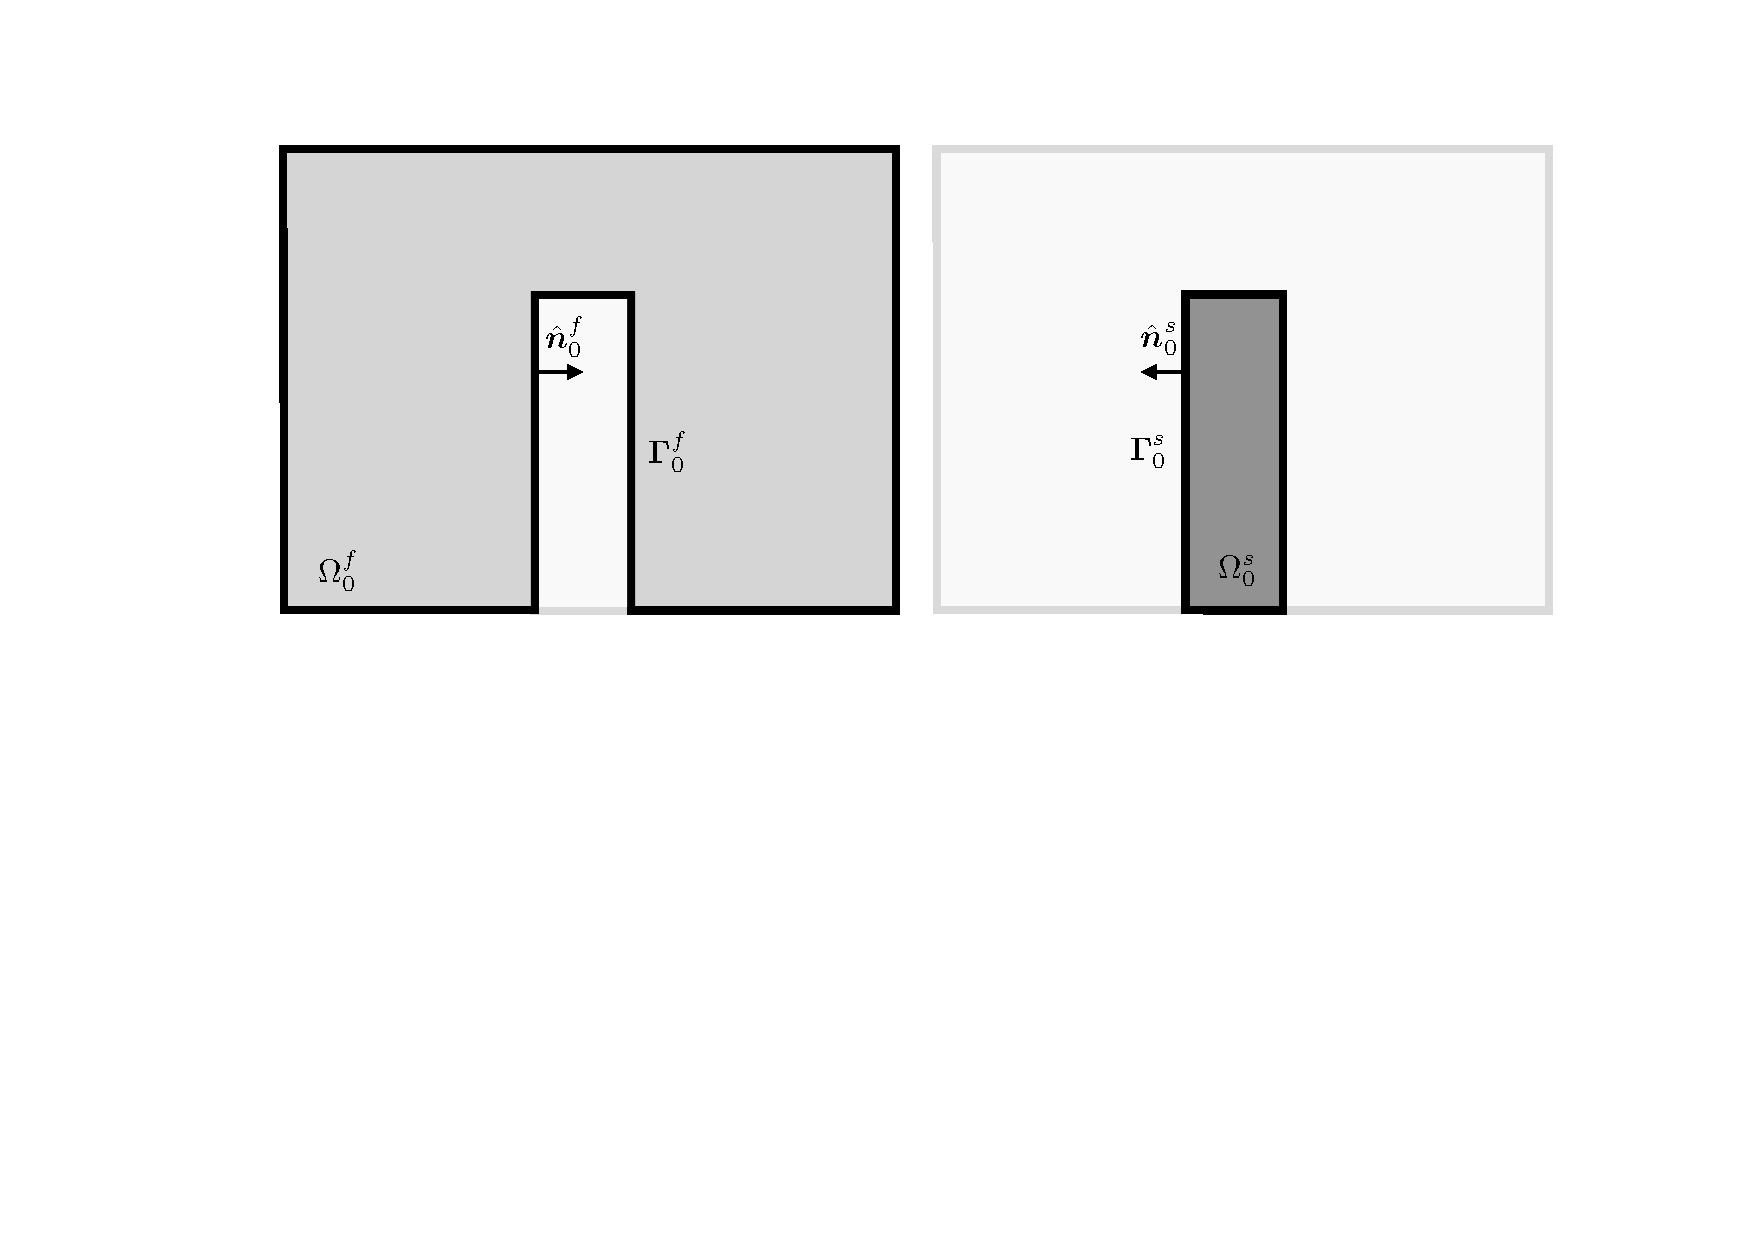
\includegraphics[width=0.8\textwidth]{figures/fsi_problem_initial} 
   	}
	\subfigure[Deformed configurations of the fluid (left) and solid (right) domains at time $t$, showing the deformed volumes $\Omega(t)$, boundaries $\bb{\Gamma}(t)$ and outward-facing unit normals $\hat{\bb{n}}(t)$]
	{
		\label{fig:mms_mesh}
   		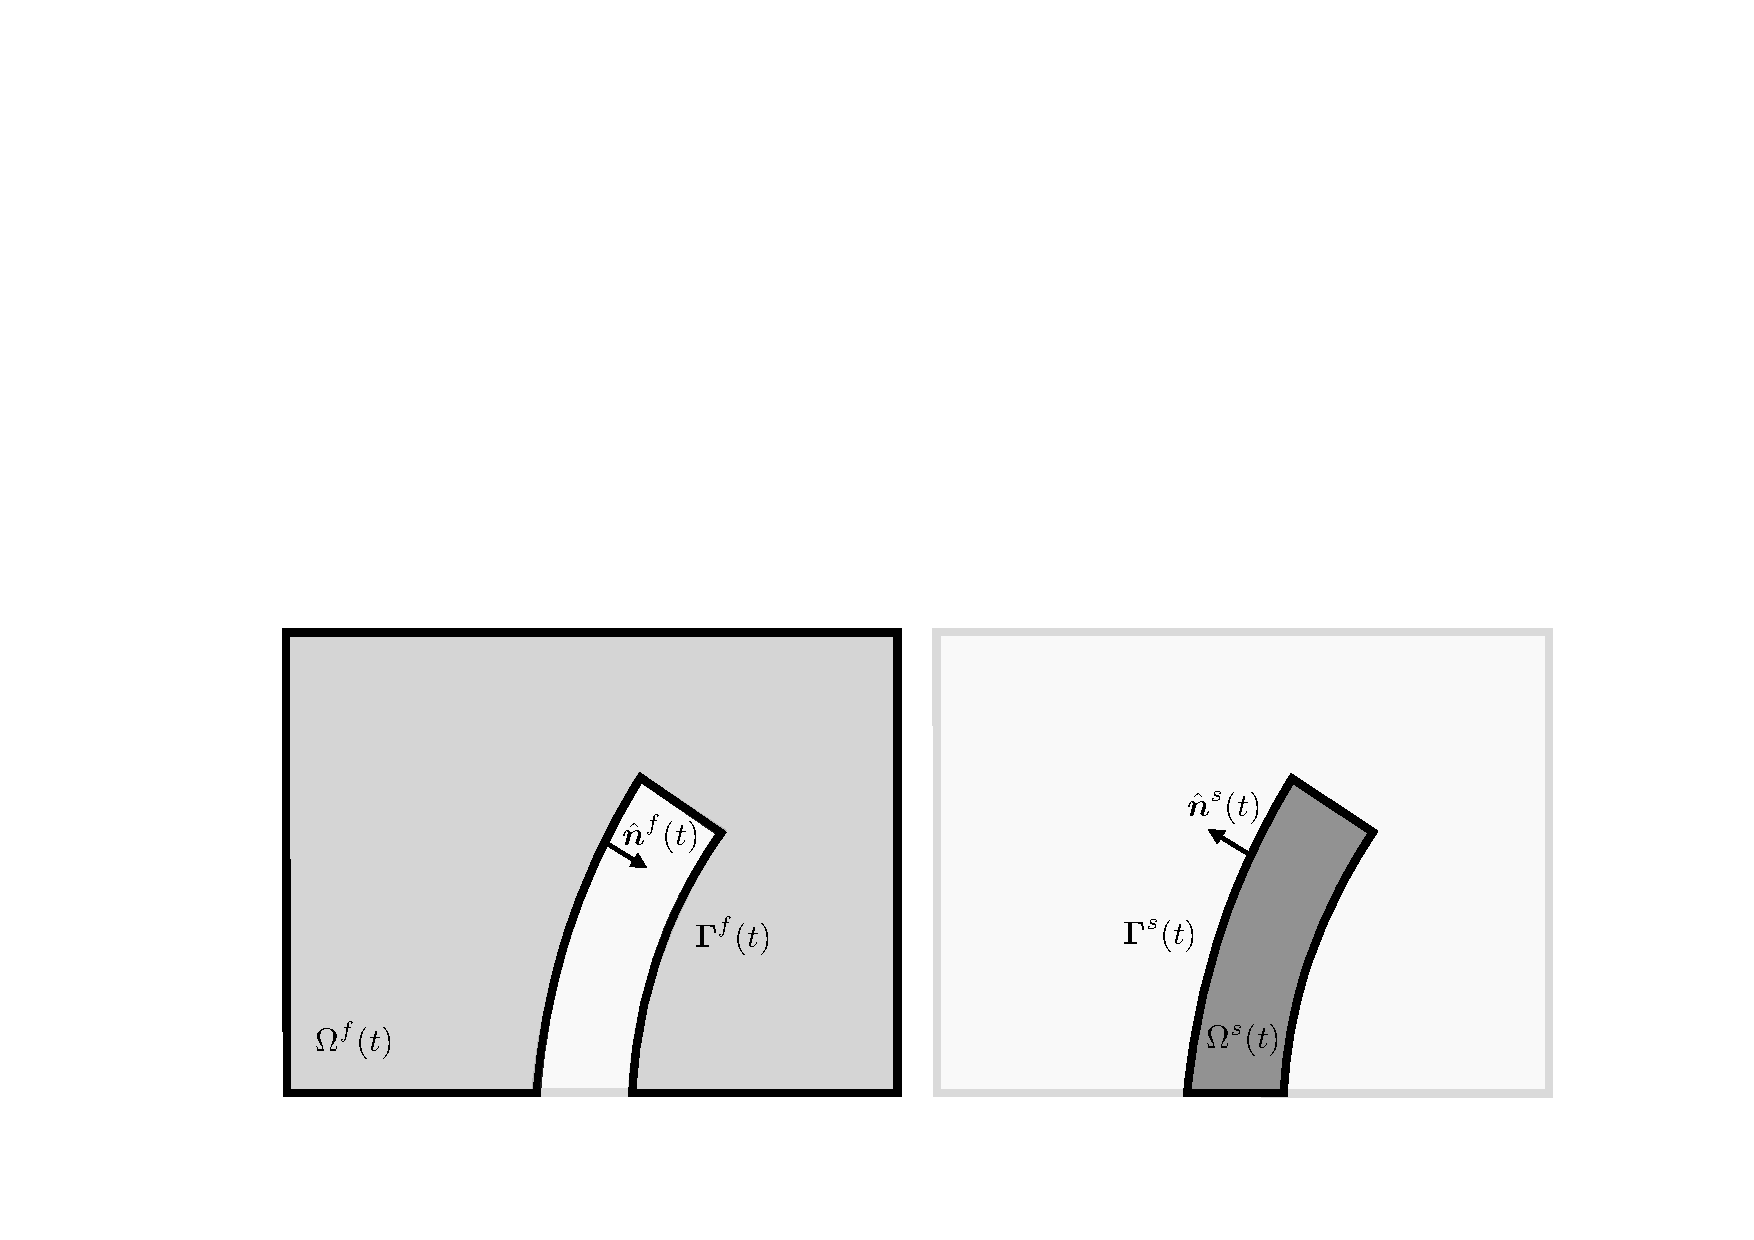
\includegraphics[width=0.8\textwidth]{figures/fsi_problem_current}  
   	}
	\caption{Representative fluid-solid interaction problem, where superscript $f$ represents fluid domain quantities and superscript $s$ represents solid domain quantities. Image adapted from \citet{OneraWebsite}}
	\label{fig:fsi_problem}
\end{figure}

OneraWebsite: https://w3.onera.fr/erc-aeroflex/en/project/strategies-for-coupling-the-fluid-and-solid-dynamics


%%%--------------------------------------------------------------------------------------------------------------------%%
%\subsection{Governing Equations in the Deformed Configurations}
%%%--------------------------------------------------------------------------------------------------------------------%%

%%----------------------------------------------------------%%
\subsection{Solid Dynamics Governing Equations}
%%----------------------------------------------------------%%
Dynamics of the solid region are governed by linear momentum conservation, which can be expressed in Lagrangian form on the deformed configuration as
\begin{eqnarray} \label{eqn:solid_momentum_deformed}
    \int_{\Omega^s} \frac{\partial \rho^s \bb{v} }{\partial t} d\Omega^s
    =
    \oint_{\Gamma^s} \hat{\bb{n}}^s \cdot \bb{\sigma} \ d\Gamma^s
    + \int_{\Omega^s}  \bb{f}_b^s \, d\Omega^s
\end{eqnarray}
where $\rho^s$ is the density, $\bb{v}^s$ is the velocity vector, $\hat{\bb{n}}^s$ is the unit outwards-facing normal to surface $\Gamma^s$, $\bb{\sigma}^s$ is the true (Cauchy) stress tensor, and $\bb{f}_b^s$ is a body force per unit volume, e.g. $\bb{f}_b^s = \rho^s \bb{g}$ for a gravity body force, where $\bb{g}$ is gravitionational acceleration.
For notational simplicity, the time dependence notation $(t)$ has been omitted from the moving volumes and surfaces; that is, $\Omega(t) \equiv \Omega$ and $\Gamma(t) \equiv \Gamma$.


%$\hat{\bb{n}}^s = \nicefrac{\bb{\Gamma}}{|\bb{\Gamma}|}$ is the outwards-pointing unit surface normal,

The integrals above (Equation \ref{eqn:solid_momentum_deformed}) are expressed over the as-yet-unknown deformed configuration. 
These integrals can be reexpressed over the known initial configuration by introducing the deformation gradient $\bb{F} = \textbf{I} + (\bb{\nabla} \bb{d})^{\text{T}}$ and its determinant as $J = \text{det}[\bb{F}]$, in terms of the displacement vector $\bb{d}$ and del operator $\bb{\nabla}$.
Note that the current work adopts the convention that $(\nabla d)_{ij} = \nicefrac{\partial d_j}{\partial x_i}$, so, to avoid confusion, $\bb{F}$ and $J$ are expressed in index notation as $F_{ij} = \delta_{ij} + \frac{\partial d_i}{\partial X_j}$ and $J = \frac{1}{6} \varepsilon_{ijk} \varepsilon_{pqr} F_{ip} F_{jq} F_{kr}$, where $\delta_{ij}$ is the Kronecker delta and $\varepsilon_{ijk}$ is the permutation symbol.

Employing $\bb{F}$ and $J$, volume integrals can be expressed over the initial configuration as
\begin{eqnarray}
    \int_{\Omega^s} \; \text{d}\Omega^s &=& \int_{\Omega_0^s} J \; \text{d}\Omega^s_0
\end{eqnarray}
From this, $J$ can be interpreted as the ratio of the deformed to the initial volume $J = \nicefrac{\Omega^s}{\Omega_0^s}$, allowing the current density to be expressed in terms of the initial density as $\rho^s = J \rho_0^s$.
Similarly, surface integrals over the deformed configuration can be reexpressed over the initial configuration as
\begin{eqnarray}
    \oint_{\Gamma^s} \hat{\bb{n}}^s \cdot \bb{\phi} \; \text{d}\Gamma^s &=&
    \oint_{\Gamma_0^s} \left(J \bb{F}^{-T} \cdot \hat{\bb{n}}_0^s \right) \cdot \bb{\phi} \; \text{d}\Gamma_0^s
\end{eqnarray}
where $\bb{\phi}$ represents an arbitrary scalar, vector or tensor field, and $\cdot$ operator is replaced by a suitable scalar/vector/tensor multiplication operator.
Here, $J \bb{F}^{-T}$ can be seen to rotate and scale the normal vector from the initial to the deformed configuration;
this stems from Nanson's relation, $\bb{\Gamma} = J \bb{F}^{-T} \cdot \bb{\Gamma}_0$, which relates the deformed area vector $\bb{\Gamma}$ to the initial area vector $\bb{\Gamma}_0$. 

With these mappings, linear momentum conservation can be expressed in the so-called \emph{total Lagrangian} form, where integrals are given over the initial configuration:
\begin{eqnarray} \label{eqn:solid_momentum_TL}
    \int_{\Omega_0^s} \rho_0 \frac{\partial^2 \bb{d} }{\partial t^2} \; d\Omega_0^s
    &=&
    \oint_{\Gamma_0^s} \left( J \bb{F}^{-\text{T}} \cdot \bb{n}_0^s \right) \cdot \bb{\sigma}^s \ d\Gamma_0^s
    + \int_{\Omega_0^s}  \bb{f}_{b_0}^s \, d\Omega_0^s
\end{eqnarray}
The body force $\bb{f}_{b_0}^s$ is per unit \emph{initial} volume, e.g. $\bb{f}_{b_0}^s = \rho^s_0 \bb{g}$.

%where $\Omega_o$ is the volume of an arbitrary body bounded by a surface $\Gamma_o$ with outwards pointing normal $\bb{n}_o$.
%Subscript $o$ indicates quantities in the initial reference configuration, which is assumed stress-free here.
%The density is $\rho$, $t$ is time, $\bb{d}$ is the displacement vector, $\bb{\sigma}$ is the true (Cauchy) stress tensor (\hl{stress is prescribed on boundary faces}), and $\bb{f}_b$ is a body force per unit volume, e.g., $\rho \bb{g}$, where $\bb{g}$ is gravity.

%The deformation gradient is defined as $\bb{F} = \textbf{I} + (\bb{\nabla} \bb{d})^{\text{T}}$ and its determinant as $J = \text{det}(\bb{F})$, or in index notation as $F_{ij} = \delta_{ij} + \frac{\partial d_i}{\partial X_j}$ and $J = \frac{1}{6} \varepsilon_{ijk} \varepsilon_{pqr} F_{ip} F_{jq} F_{kr}$.

The definition of the true stress ($\bb{\sigma}^s$ in Equations \ref{eqn:solid_momentum_deformed} and \ref{eqn:solid_momentum_TL}) is given by a chosen mechanical law.
Four mechanical laws are considered in this work, as defined in Appendix A of \citet{Cardiff2025JFNK}: linear elasticity (Hooke's law), and three forms of hyperelasticity (St.\ Venant-Kirchhoff, neo-Hookean, and Guccione).
%\hl{We may need to mention linear elasticity, depending on the test case - or not}

Three types of boundary conditions for the solid domain are considered here: prescribed displacement, prescribed traction, and symmetry.

%The displacement increment is the change in displacement between the current time step and the previous time step when the time interval is discretised into a finite number of steps.



%%--------------------------------------------------------------------------------------------------------------------%%
\subsection{Fluid Dynamics Governing Equations} \label{sec:fluid_governing_eqn}
%%--------------------------------------------------------------------------------------------------------------------%%

The dynamics of the moving fluid region are governed by mass conservation and linear momentum conservation.
%, which can be expressed in Lagrangian form on the deformed configuration as
%
%An arbitrary Lagrangian-Eulerian (ALE) formulation is adopted for the fluid formulation in the current, defined by mass continuity, linear momentum conservation, and space conservation.
Mass continuity is equivalent to volume continuity for an incompressible material and can be expressed for a moving domain as
\begin{eqnarray} \label{eqn:continuity_deformed_full}
	\frac{d}{dt} \int_{\Omega^f} \, d\Omega^f
	\;+\; \oint_{ \Gamma^f} \hat{\bb{n}}^f \cdot (\bb{v}^f - \boldsymbol{v}^{\Gamma}) \, d\Gamma^f = 0
\end{eqnarray}
where $\bb{v}^f$ is the fluid velocity, and $\boldsymbol{v}^\Gamma$ is the velocity of the moving surface $\Gamma^f$.
%$\Omega$ is the volume of an arbitrary body bounded by a surface $\Gamma$ with outwards pointing normal $\bb{n}$,
The continuity equation simplifies to
\begin{eqnarray} \label{eqn:continuity_deformed}
	\oint_{ \Gamma^f} \hat{\bb{n}}^f \cdot \bb{v}^f \, d\Gamma^f = 0
\end{eqnarray}
by using the geometric (space) conservation law
\begin{eqnarray} \label{eqn:space_conservation}
	\frac{d}{dt} \int_{\Omega^f} \, d\Omega^f
	\; - \; \oint_{ \Gamma^f} \hat{\bb{n}}^f \cdot \boldsymbol{v}^\Gamma \, d\Gamma^\Gamma = 0
\end{eqnarray}
%which states that the rate of change of the fluid domain volume (or a subset of it) must equal the net flux of the velocity across its boundaries.


Similarly, linear momentum can be expressed in Eulerian form for a laminar, Newtonian, incompressible, isothermal fluid in a moving domain as
\begin{eqnarray} \label{eqn:momentum_fluid_deformed}
	\frac{d}{dt} \int_{\Omega^f} \bb{v}^f \, d\Omega^f
	+ \oint_{\Gamma^f} \hat{\bb{n}}^f \cdot (\bb{v}^f - \bb{v}^\Gamma) \boldsymbol{v}^f \, d\Gamma^f
	=  \oint_{\Gamma^f} \hat{\bb{n}}^f \cdot \bb{\sigma}^f \, d\Gamma^f
%	=  \oint_{\Gamma^f} \hat{\bb{n}}^f \cdot \left(\nu \bb{\nabla} \bb{v}^f \right) \, d\Gamma^f
%%	+ \frac{1}{\rho} \int_{\Omega} \bb{\nabla} p \, d\Omega
%	+ \int_{\Omega^f} \bb{\nabla} p \, d\Omega^f
	+ \int_{\Omega^f} \bb{f}_b^f \, d\Omega^f
\end{eqnarray}
where $\bb{f}_b^f$ are body forces per mass, e.g., $\bb{f}_b^f = g$.
The true (Cauchy) stress $\bb{\sigma}^f$ is defined for a Newtonian fluid as
\begin{eqnarray} \label{eqn:fluid_stress}
	\bb{\sigma}^f &=& \nu \bb{\nabla} \bb{v}^f + \nu \left(\bb{\nabla} \bb{v}^f \right)^T - p \textbf{I}
\end{eqnarray}
where $\nu$ is the kinematic viscosity, $p$ is the kinematic pressure (pressure per density), and $\textbf{I}$ is the second-order identity tensor.
%\begin{eqnarray} \label{eqn:momentum_fluid_deformed}
%	\frac{d}{dt} \int_{\Omega^f} \bb{v}^f \, d\Omega^f
%	+ \oint_{\Gamma^f} \hat{\bb{n}}^f \cdot (\bb{v}^f - \bb{v}^\Gamma) \boldsymbol{v}^f \, d\Gamma^f
%	=  \oint_{\Gamma^f} \hat{\bb{n}}^f \cdot \left(\nu \bb{\nabla} \bb{v}^f \right) \, d\Gamma^f
%%	+ \frac{1}{\rho} \int_{\Omega} \bb{\nabla} p \, d\Omega
%	+ \int_{\Omega^f} \bb{\nabla} p \, d\Omega^f
%%	+ \int_{\Omega} \boldsymbol{f} \, d\Omega
%\end{eqnarray}
%where $\nu$ is the kinematic viscosity, $p$ is the kinematic pressure (pressure per density), and other body forces, such as gravity, are neglected here.
%$\rho$ is the density, 

As was the case for the solid dynamics equations, the integrals above (Equations \ref{eqn:continuity_deformed} and \ref{eqn:momentum_fluid_deformed}) are expressed over the unknown deformed fluid configuration and must be expressed over a known configuration.
To achieve this, we employ the deformation gradient $\bb{F}^{\Gamma}$ for the moving fluid domain; that is, the deformation of the fluid domain is driven by the motion of the fluid-solid interface, where, as yet, we have not defined a governing equation for the propagation of this interface motion into the fluid domain.
For a given fluid domain displacement $\bb{d}^{\Gamma}$, the fluid domain deformation gradient is defined as $\bb{F}^{\Gamma} = \textbf{I} + (\bb{\nabla} \bb{d}^\Gamma)^{\text{T}}$ and its determinant as $J^\Gamma = \text{det}[\bb{F}^\Gamma]$.

Employing $\bb{F}_{\Gamma}$ and $J_\Gamma$, volume continuity can be expressed in terms of an integral over the initial fluid configuration as
\begin{eqnarray} \label{eqn:continuity_initial}
%	\oint_{\Gamma^f_0}  \left( J \bb{F}^{-\text{T}} \cdot \hat{\bb{n}}_0^s \right)  \cdot (\bb{v}^f - \boldsymbol{v}^{\Gamma}) \, d\Gamma^f_0 = 0
	\oint_{\Gamma^f_0}  \left( J \bb{F}^{-\text{T}} \cdot \hat{\bb{n}}_0^f \right) \cdot \bb{v}^f \, d\Gamma^f_0 = 0
\end{eqnarray}

Before expressing linear momentum conservation over the initial configuration, we must introduce the mapping of the gradient operator in the deformed configuration to the gradient operator in the initial configuration:
\begin{eqnarray}
	\bb{\nabla} \bb{\phi} = \bb{F}^{-T} \cdot \left( \bb{\nabla}_0 \bb{\phi} \right) \\
	\left( \bb{\nabla} \bb{\phi} \right)^T = \left( \bb{\nabla}_0 \bb{\phi} \right)^T \cdot  \bb{F}^{-1} 
\end{eqnarray}

With these mappings, linear momentum conservation for the fluid can be expressed over the initial configuration as
%\begin{eqnarray} \label{eqn:momentum_fluid_deformed}
%	\int_{\Omega^f_0} J_\Gamma \frac{\partial \bb{v}^f}{\partial t} \, d\Omega^f_0
%	+ \oint_{\Gamma^f_0}  \left( J \bb{F}^{-\text{T}} \cdot \bb{n}_0^s \right) \cdot (\bb{v}^f - \bb{v}_\Gamma) \boldsymbol{v}^f \, d\Gamma^f_0
%	= \notag \\
%	 \oint_{\Gamma^f_0}  \left( J \bb{F}^{-\text{T}} \cdot \bb{n}_0^s \right) \cdot \left[\nu \bb{F}^{-T} \cdot \left( \bb{\nabla}_0 \bb{v}^f \right) \right] \, d\Gamma^f_0
%	+ \int_{\Omega^f_0} J_\Gamma \bb{F}^{-T} \cdot \left( \bb{\nabla}_0 p \right) \, d\Omega^f_0
%\end{eqnarray}
\begin{align} \label{eqn:momentum_fluid_deformed}
\int_{\Omega^f_0} J^\Gamma \frac{\partial \bb{v}^f}{\partial t} \, d\Omega^f_0
	&+ \oint_{\Gamma^f_0}  \left[ J^\Gamma (\bb{F}^\Gamma)^{-\text{T}} \cdot \hat{\bb{n}}_0^f \right] \cdot \left(\bb{v}^f - \frac{\partial \bb{d}^\Gamma}{\partial t}\right) \bb{v}^f \, d\Gamma^f_0 = \notag \\
	&\oint_{\Gamma^f_0}  \left[ J^\Gamma (\bb{F}^\Gamma)^{-\text{T}} \cdot \hat{\bb{n}}_0^f \right]
	\cdot \left[\nu (\bb{F}^\Gamma)^{-T} \cdot \left( \bb{\nabla}_0 \bb{v}^f \right) \right] \, d\Gamma^f_0 \notag \\
	&\quad + \int_{\Omega^f_0} J^\Gamma (\bb{F}^\Gamma)^{-T} \cdot \left( \bb{\nabla}_0 p \right) \, d\Omega^f_0
\quad+\quad \int_{\Omega^f_0} \bb{f}_{b_0}^f \, d\Omega^f_0
\end{align}
where the time derivative in the first term is brought inside the integral as the initial volume is unchanging.
In addition, the identity
$\bb{\nabla} \cdot \left[ \left(\bb{\nabla} \bb{v}^f \right)^T \right] = \bb{\nabla} \left( \bb{\nabla} \cdot \bb{v}^f \right) = \bb{0}$ has been employed, and the velocity $\bb{v}^\Gamma$ of the moving fluid domain has been replaced with the time derivative $\nicefrac{\partial \bb{d}^\Gamma}{\partial t}$ of the moving fluid domain displacement.

For the fluid domain, four boundary condition types are considered: inlet, outlet, no-slip wall, and symmetry.


%%--------------------------------------------------------------------------------------------------------------------%%
\subsection{Fluid-Solid Interface Conditions} \label{sec:fsi_interface}
%%--------------------------------------------------------------------------------------------------------------------%%
At the interface $\Gamma_\text{fsi}$ between the solid and fluid regions, mass conservation leads to the \emph{kinematic} interface conditions, which state that the velocity of the fluid is equal to the velocity of the solid and the velocity of the moving fluid domain:
\begin{eqnarray} \label{eqn:kinematic}
	\bb{v}^f = \frac{\partial \bb{d}^s}{\partial t} = \frac{\partial \bb{d}^\Gamma}{\partial t}
	\quad\quad\quad\quad\text{on}\quad \Gamma_\text{fsi}
\end{eqnarray}
ensuring the fluid and solid share the same motion at the interface (i.e., there is no gap or overlap), assuming the fluid and solid interfaces are coincident in the initial configuration.

%Subscripts $f$ and $s$ are introduced to indicate fluid and solid quantities, respectively.

Linear momentum conservation yields the \emph{kinetic} interface condition in the deformed configuration $\Gamma_\text{fsi}$ as:
\begin{eqnarray} \label{eqn:kinetic_deformed}
	\hat{\bb{n}}^f \cdot \bb{\sigma}^f &=& -\hat{\bb{n}}^s \cdot \bb{\sigma}^s \\
	\hat{\bb{n}}^f \cdot \left[\nu \bb{\nabla} \bb{v}^f + \nu \left(\bb{\nabla} \bb{v}^f \right)^T - p \right]
		&=& -\hat{\bb{n}}^s \cdot \bb{\sigma}^s
\end{eqnarray}
where $\hat{\bb{n}}^f = -\hat{\bb{n}}^s$, as the surface normals are assumed to point outwards from each region.
Equivalently, the kinetic condition can be expressed on the initial configuration as
\begin{eqnarray} \label{eqn:kinetic_initial}
	\left[ J^\Gamma (\bb{F}^\Gamma)^{-\text{T}} \cdot \hat{\bb{n}}_0^f \right] \cdot \bb{\sigma}^f &=&
	-\left[ J \bb{F}^{-\text{T}} \cdot \hat{\bb{n}}_0^s \right] \cdot \bb{\sigma}^s \\
	\left[ J^\Gamma (\bb{F}^\Gamma)^{-\text{T}} \cdot \hat{\bb{n}}_0^f \right]
	 \cdot 
	 \left[
	 \nu (\bb{F}^\Gamma)^{-T} \cdot \bb{\nabla} \bb{v}^f 
	 + \nu \left(\bb{\nabla} \bb{v}^f \right)^T \cdot (\bb{F}^\Gamma)^{-1}
	 - p
	 \right]
	&=& 
	-\left[ J \bb{F}^{-\text{T}} \cdot \hat{\bb{n}}_0^s \right] \cdot \bb{\sigma}^s
\end{eqnarray}


%%--------------------------------------------------------------------------------------------------------------------%%
\subsection{Fluid Domain Motion} \label{sec:fluid_domain_motion}
%%--------------------------------------------------------------------------------------------------------------------%%
The motion of the fluid-solid interface $\Gamma_\text{fsi}$ is dictated by the motion of the solid domain; however, as yet, we have not defined how this interface motion should be distributed throughout the fluid domain.
This fluid domain motion need not follow a conservation law and should instead be ideally defined to smoothly transit the interface motion, preserving the quality of the computational mesh—to be described below.
Nonetheless, any chosen fluid domain motion procedure or equation should follow the geometric (space) conservation law (Equation \ref{eqn:space_conservation}), 
which states that the rate of change of the fluid domain volume (or a subset of it) must equal the net flux of the domain velocity across its boundaries.
%\begin{eqnarray} \label{eqn:space_conservation}
%	\frac{d}{dt} \int_{\Omega^f} \, d\Omega^f
%	\; - \; \oint_{ \Gamma^f} \hat{\bb{n}}^f \cdot \boldsymbol{v}^\Gamma \, d\Gamma^\Gamma = 0
%\end{eqnarray}

In the current work, the displacement $\bb{d}^\Gamma$ of the fluid domain is assumed to follow the pseudo-solid linear elastic, static momentum equation:
\begin{eqnarray} \label{eqn:motion_momentum}
%    \oint_{\Gamma_0^f} \left( J^\Gamma (\bb{F}^\Gamma)^{-\text{T}} \cdot \bb{n}_0^f \right) \cdot \bb{\sigma}^\Gamma \ d\Gamma_0^f
    \oint_{\Gamma_0^f} \bb{n}_0^f \cdot
    \left[
    \mu^\Gamma \bb{\nabla}_0 \bb{d}^\Gamma + \mu^\Gamma \left(\bb{\nabla}_0 \bb{d}^\Gamma\right)^T
    + \lambda^\Gamma (\bb{\nabla}_0 \cdot \bb{d}^\Gamma) \textbf{I}
    \right]
    \, d\Gamma_0^f
    &=& \bb{0}
\end{eqnarray}
where $\mu^\Gamma$ and $\lambda^\Gamma$ are spatially-varying \emph{stiffness} parameters for controlling the distribution of the motion.
Note that the quantities are not mapped to the deformed configuration, resulting in the equation being linear in $\bb{d}^\Gamma$; as a result, this approach does not formally conserve linear momentum, however, as will be shown in test cases section below, it is sufficient for maintaining the fluid domain computational mesh quality.
The value of $\bb{d}^\Gamma$ is prescribed on all boundaries of $\Gamma^f$, where the $\bb{d}^\Gamma = \bb{d}^s$ on the fluid-solid interface and zero on other boundaries.




%%%--------------------------------------------------------------------------------------------------------------------%%
%\subsection{Boundary Conditions} \label{sec:BCs}
%%%--------------------------------------------------------------------------------------------------------------------%%
%\hl{Maybe mention these in passing in the sections above when giving the governing equations}
%\hl{Also, I need to mention the material/space the eqns apply to}
%Three types of boundary conditions for the solid domain are considered here: prescribed displacement, prescribed traction, and symmetry.
%For the fluid domain, four boundary condition types are considered: inlet, outlet, no-slip wall, and symmetry.
%\hl{Give math definitions}


%%%%%%%%%%%%%%%%%%%%%%%%%%%%%%%%%%%%%%%%%%%%%%%%%%%%%%%%%%%%%
\section{Numerical Methods}\label{sec:numerical_methods}
%%%%%%%%%%%%%%%%%%%%%%%%%%%%%%%%%%%%%%%%%%%%%%%%%%%%%%%%%%%%%

%%--------------------------------------------------------------------------------------------------------------------%%
\subsection{Spatio-temporal Discretisation}
\label{sec:space_time_discretisation}
%%--------------------------------------------------------------------------------------------------------------------%%
The solution domain is discretised in both space and time.
The total simulation period is divided into a finite number of time increments, denoted as $\Delta t$, and the discretised governing equations are solved iteratively in a time-marching fashion.
The fluid and solid spatial domains are partitioned into a finite set $\mathcal{P}$ of contiguous convex polyhedral cells, where each cell is denoted by $P \in \mathcal{P}$.
The total number of cells in the mesh is indicated by $|\mathcal{P}| = |\mathcal{P}|^f + |\mathcal{P}^s|$, where $|\mathcal{P}^f|$ indicates the number of cells in the fluid mesh and $|\mathcal{P}^s|$ indicates the number in the solid mesh.
A representative cell $P$ is shown in Figure~\ref{fig:cell}.
The set of all faces of cell $P$ is denoted by $\mathcal{F}_P$. This set is further subdivided into three disjoint subsets:
\begin{itemize}
    \item \textbf{Internal Faces} ($\mathcal{F}^{\text{int}}_P$): Faces that are shared with neighbouring cells, excluding the fluid-solid interface. 
    \item \textbf{Boundary Faces} ($\mathcal{F}^{\text{bnd}}_P$): Faces that lie on the boundary of the spatial domain, excluding the fluid-solid interface.
    %The boundary faces of cell $P$ are further classed into three disjoint sets, $\mathcal{F}^{\text{bnd}}_P \coloneqq \mathcal{F}^{\text{disp}}_P \cup \mathcal{F}^{\text{trac}}_P \cup \mathcal{F}^{\text{symm}}_P$, representing boundary faces where displacement ($\mathcal{F}^{\text{disp}}_P$), traction ($\mathcal{F}^{\text{trac}}_P$) and symmetry ($\mathcal{F}^{\text{symm}}_P$) conditions are prescribed.
    %\hl{include fluid}
       % \quad \text{with} \quad \mathcal{F}^{\text{disp}}_P \cap \mathcal{F}^{\text{trac}}_P = \mathcal{F}^{\text{disp}}_P \cap \mathcal{F}^{\text{symm}}_P = \mathcal{F}^{\text{trac}}_P \cap \mathcal{F}^{\text{symm}}_P = \emptyset.$
    \item \textbf{Fluid-Solid Interface Faces} ($\mathcal{F}^{\text{fsi}}_P$): Faces that lie on the fluid-solid interface; that is, faces that straddle a cell in the fluid mesh and a cell in the solid mesh.
\end{itemize}

\hl{I need to update below: notation becomes too verbose when FSI is added}
\hl{Maybe include as internal face and introduce notation for subsets}
Each internal face $f_i \in \mathcal{F}^{\text{int}}_P$ corresponds to a neighbouring cell $N_{f_i} \in \mathcal{N}_P$, where $\mathcal{N}_P$ is the set of all neighbouring cells of $P$ in the same region. The outward unit normal vector associated with an internal face $f_i$ is denoted by $\mathbf{n}_{f_i}$, while $\mathbf{n}_{b_i}$ indicates the normal for a boundary face $b_i$, and $\mathbf{n}_{I_i}$ indicates the normal for a fluid-solid interface face $I_i$.
The vector $\mathbf{d}_{f_i}$ connects the centroid of cell $P$ with the centroid of the neighbouring cell $N_{f_i}$, whereas the vector $\mathbf{d}_{b_i}$ connects the centroid of cell $P$ with the centroid of boundary face ${b_i}$, and the vector $\mathbf{d}_{I_i}$ connects the centroid of cell $P$ with the centroid of the neighbouring cell $N_{I_i}$ across a fluid-solid interface.
%For convenience, we will also define the set of all faces of cell $P$ excluding those on a traction boundary as $\mathcal{F}_P^{\text{non-trac}} \coloneqq \mathcal{F}_P^{\text{int}} \cup \mathcal{F}_P^{\text{disp}} \cup \mathcal{F}_P^{\text{symm}}$.
\begin{figure}[htbp]
	\centering
   		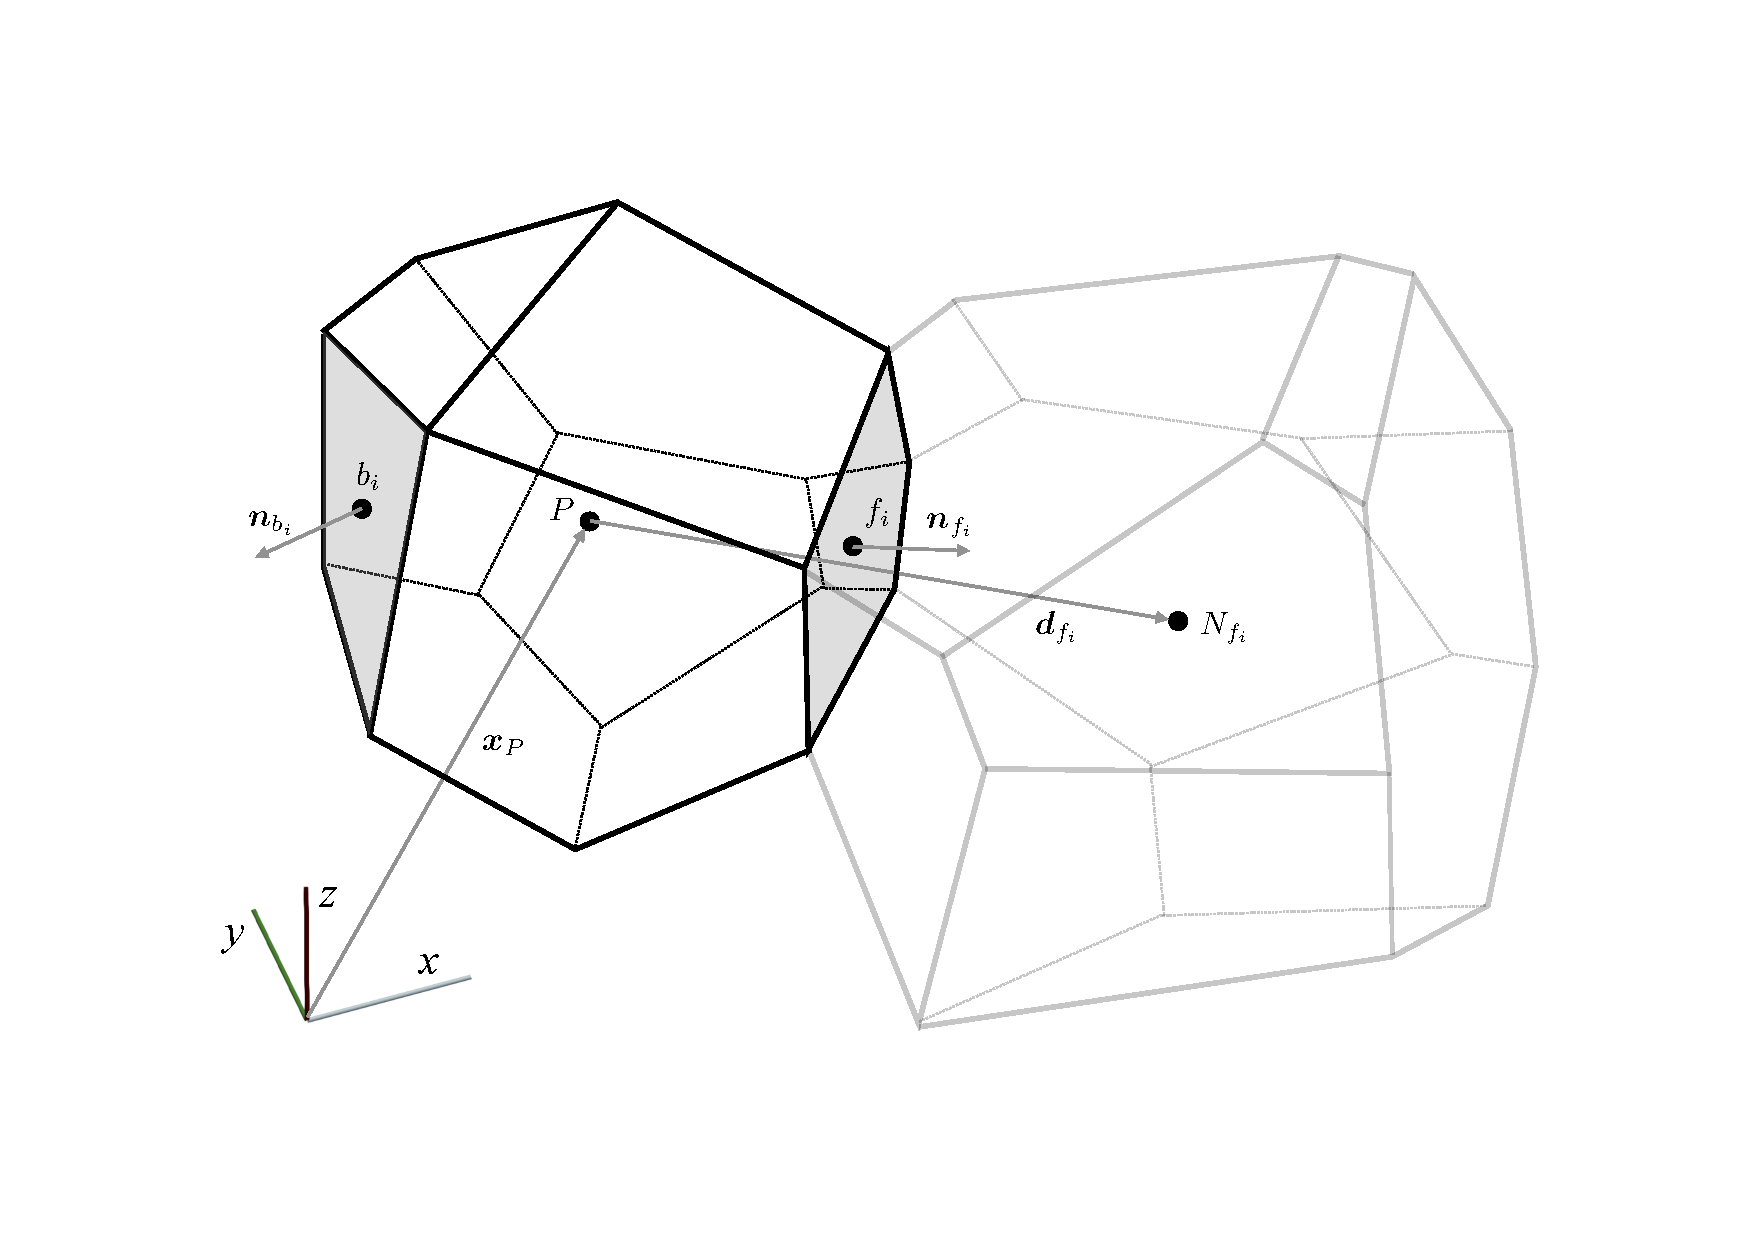
\includegraphics[width=0.8\textwidth]{figures/cell} 
	\caption{Representative convex polyhedral cell $P$ and neighbouring cell $N_{f_i}$, which share a face $f_i$ (Taken from \citet{Cardiff2025:JFNK})}
	\label{fig:cell}
\end{figure}







%%--------------------------------------------------------------------------------------------------------------------%%
\subsection{Newton-Type Solution Method}
%%--------------------------------------------------------------------------------------------------------------------%%
To facilitate the application of a Newton-type solution algorithm, the governing equations are expressed in \emph{residual} form as:
\begin{eqnarray} \label{eqn:residual}
	    \bb{R}(\bb{U}) =
	         \begin{pmatrix}
			\bb{R}_u  \\
			R_p \\
			\bb{R}_m \\
		    	\bb{R}_d
		    \end{pmatrix}
		= \bb{0}
\end{eqnarray}
where $\bb{R}$ represents the \emph{residual} (imbalance) of the equations, which is a function of the primary unknowns field $\bb{U} = \left\{\bb{v}, p, \bb{d}_m, \bb{d} \right\}$.
Concretely, the components of the residual are given as \hl{use on Omega f notation etc}
\begin{eqnarray} \label{eq:residuals}
    \bb{R}_u %(\bb{U})
    &=&
	\oint_{\Gamma^f_0}  \left[ J^\Gamma (\bb{F}^\Gamma)^{-\text{T}} \cdot \hat{\bb{n}}_0^f \right]
		\cdot \left[\nu (\bb{F}^\Gamma)^{-T} \cdot \left( \bb{\nabla}_0 \bb{v}^f \right) \right] \, d\Gamma^f_0
	+ \int_{\Omega^f_0} J^\Gamma (\bb{F}^\Gamma)^{-T} \cdot \left( \bb{\nabla}_0 p \right) \, d\Omega^f_0 \notag \\
	&&+ \int_{\Omega^f_0} \bb{f}_{b_0}^f \, d\Omega^f_0
	- \int_{\Omega^f_0} J^\Gamma \frac{\partial \bb{v}^f}{\partial t} \, d\Omega^f_0 
	- \oint_{\Gamma^f_0}  \left[ J^\Gamma (\bb{F}^\Gamma)^{-\text{T}} \cdot \hat{\bb{n}}_0^f \right] \cdot \left(\bb{v}^f - \frac{\partial \bb{d}_m}{\partial t}\right) \bb{v}^f \, d\Gamma^f_0
	\notag \\
	&&+\; \bb{\mathcal{D}}_v
	\notag \\
    R_p %(\bb{U})
    &=&	\oint_{\Gamma^f_0}  \left[ J^\Gamma (\bb{F}^\Gamma)^{-\text{T}}  \cdot \hat{\bb{n}}_0^f \right] \cdot \bb{v}^f \, d\Gamma^f_0 \;+\; \mathcal{D}_p
    \notag \\
    \bb{R}_m
    &=&
    \oint_{\Gamma_0^f} \bb{n}_0^f \cdot
    \left[
    \mu^\Gamma \bb{\nabla}_0 \bb{d}_m + \mu^\Gamma \left(\bb{\nabla}_0 \bb{d}_m \right)^T
    + \lambda^\Gamma (\bb{\nabla}_0 \cdot \bb{d}_m) \textbf{I}
    \right]
    \, d\Gamma_0^f
    \;+\; \bb{\mathcal{D}}_m
    \notag \\
    \bb{R}_d %(\bb{U})
    &=&
    \oint_{\Gamma_0^s} \left( J \bb{F}^{-\text{T}} \cdot \bb{n}_0^s \right) \cdot \bb{\sigma}^s \ d\Gamma_0^s
    + \int_{\Omega_0^s}  \bb{f}_{b_0}^s \, d\Omega_0^s
    - \int_{\Omega_0^s} \rho_0 \frac{\partial^2 \bb{d} }{\partial t^2} \; d\Omega_0^s
    \;+\; \bb{\mathcal{D}}_d
\end{eqnarray}
where $\bb{\mathcal{D}}_v$, $\mathcal{D}_p$, $\bb{\mathcal{D}}_m$, and $\bb{\mathcal{D}}_d$ are stabilisation terms to be defined.

The residuals $\bb{R}_v$, $R_p$ and $\bb{R}_m$ are applied to each cell in the fluid domain and discretised, while residual $\bb{R}_d$ is applied to each cell in the solid domain and discretised, as is described below.
The resulting system of coupled nonlinear equations in terms of $\bb{U}$ can be linearised and iteratively solved using a Newton-type method:
%In Newton-type methods, a Taylor expansion about a current point $\bb{u}_k$ can be used to solve Equation \ref{eqn:residual} \cite{Knoll2004}:
%\begin{eqnarray}
%	\bb{R}(\bb{u}_{k+1}) = \bb{R}(\bb{u}_{k}) \;+\;  \bb{R}'(\bb{u}_{k}) (\bb{u}_{k+1} - \bb{u}_{k}) \;+\; \text{H.O.T.} = \bb{0}
%\end{eqnarray}
%Neglecting the higher-order terms ($\text{H.O.T.}$) yields the strict Newton method in terms of an iteration over a sequence of linear systems: 
\begin{eqnarray} \label{eq:NewtonRaphson}
	\bb{J}(\bb{U}_k) \delta \bb{U} &=& -\bb{R}(\bb{U}_k), \notag \\
	\bb{U}_{k+1} &=& \bb{U}_k + s \, \delta \bb{U}, \notag \\
	\quad
	k &=& 0,1,...
\end{eqnarray}
where $\bb{J} \equiv \bb{R}' \equiv \partial \bb{R}/\partial \bb{U}$ is the Jacobian matrix.
Starting the Newton procedure requires the specification of $\bb{U}_0$.
%is iteratively solved by linearisation about the current value of the solution, leading to a linear system and iterative update of the solution vector:
%\begin{eqnarray}
%    \label{eq:NewtonRaphsonA}
%    \overbrace{\left[ \frac{\partial \mathcal{R}(\bb{u})}{\partial \bb{u}} \right]_n}^{\mathcal{J}} \Delta \bb{u} = -\mathcal{R}(\bb{u})_n \\
%    \label{eq:NewtonRaphsonB}
%    \bb{u}_{n+1} = \bb{u}_{n} + \alpha \Delta \bb{u}
%\end{eqnarray}
%where subscript $n$ indicates the outer (Newton) iteration index.
The scalar $s > 0$ can be chosen to improve convergence, for example, using a line search or under-relaxation/damping procedure, and is equal to unity in the classic Newton-Raphson approach.
Iterations are performed over this system until the residual $\bb{R}(\bb{U}_k)$ and solution correction $\delta \bb{U}$ are sufficiently small, with appropriate normalisation.

The linear system in Equation \ref{eq:NewtonRaphson} can be represented as
\begin{eqnarray} \label{eqn:jacobian}
\begin{bmatrix}
%\bb{J}_{vv} & \bb{J}_{vp} & \bb{J}_{vm} & \bb{J}_{vd} \\
%J_{pv} & J_{pp} & J_{pm} & J_{pd} \\
\bb{J}_{vv} & \bb{J}_{vp} & \bb{J}_{vm} & 0 \\
J_{pv} & J_{pp} & J_{pm} & 0 \\
0 & 0 & \bb{J}_{mm} & \bb{J}_{md} \\
\bb{J}_{dv} & \bb{J}_{dp} & 0 & \bb{J}_{dd}
\end{bmatrix}_k
\begin{bmatrix}
\delta \bb{v} \\
\delta p \\
\delta \bb{d}_m \\
\delta \bb{d}
\end{bmatrix}
=
-
\begin{bmatrix}
\bb{R}_v  \\
R_p \\
\bb{R}_m \\
\bb{R}_d
\end{bmatrix}_k
\end{eqnarray}
where the subscript $k$ indicates that the Jacobian matrix and right-hand side vector are evaluated in terms of $\bb{U}_k$.
\hl{Jvd and Jpd can be removed since this comes form Jvm and Jpm}
The submatrices $\bb{J}_{ab}$ represent the coupling in the residual $a$ coming from the unknown $b$.
Several types of coupling exist between the residual components:
\begin{itemize}
	\item \textbf{Fluid-to-solid}, represented by $\bb{J}_{dv}$ and $\bb{J}_{dp}$:
	the fluid forces are passed to the solid by replacing the solid stress $\bb{\sigma}^s$ with the fluid stress $\bb{\sigma}^f$ at the fluid-solid interface in $\bb{R}_d$.
	\item \hl{Merge with below}  \textbf{Solid-to-fluid}, represented by $\bb{J}_{vd}$ and $\bb{J}_{pd}$ \hl{not required, per se}
	the solid motion is passed to the fluid equations by replacing the fluid velocity $\bb{v}^f$ by the solid velocity $\nicefrac{\partial \bb{d}^s}{\partial t}$ at the fluid-solid interface in $\bb{R}_v$ and $R_p$.
	\item \textbf{Solid-to-mesh}, represented by $\bb{J}_{md}$:
	the solid motion is passed to the fluid mesh by replacing the fluid mesh displacement $\bb{d}_m$ by the solid displacement $\bb{d}^s$ at the fluid-solid interface in $\bb{R}_m$. 
	\item \hl{Rename} \textbf{Mesh-to-fluid}, represented by $\bb{J}_{vm}$ and $\bb{J}_{pm}$:
	the fluid mesh motion velocity $\nicefrac{\partial \bb{d}_m}{\partial t}$ appears in the advection term of $\bb{R}_v$ and the fluid mesh motion displacement $\bb{d}_m$ appears in the fluid mesh deformation gradients terms ($\bb{F}_m$, $J_m$) of $\bb{R}_v$ and $R_p$.
\end{itemize}
Several submatrices are not present, indicating an absence of coupling:
\begin{itemize}
	\item $\bb{J}_{mv}$, $\bb{J}_{mp}$: the fluid mesh motion $\bb{d}_m$ does not depend on the fluid velocity $\bb{v}$ and pressure $p$.
	\item $\bb{J}_{dm}$: the solid motion $\bb{d}$ does not depend on the fluid mesh motion $\bb{d}_m$. 
\end{itemize}

The current work adopts a Jacobian-free Newton-Krylov solution procedure \citep{Cardiff2025JFNK} to solve the nonlinear system given by Equation \ref{eqn:residual}.
Consequently, the true Jacobian given in Equation \ref{eqn:jacobian} is not strictly required; instead, an approximate Jacobian $\tilde{\bb{J}}$ is formed and employed to precondition the nonlinear Newton-Krylov solution.
Note that adopting an approximate Jacobian does not affect the final converged solution in each time step, assuming convergence is achieved; in addition, the quadratic convergence of the Newton-Raphson method is unaffected, once again assuming convergence is achieved.
Instead, this approximate Jacobian only affects the convergence of the linear iterative (Krylov) solver.
Others have proposed the use of physics-specific preconditioning procedures, e.g. \citet{Gee20??_Wall} and \citet{Heil2008} => these approaches sound better, but here we use a simpler approach to demonstrate the first FVM monolithic FSI solver.
Physics preconditioners are certainly suitable (e.g., using SIMPLE and segregated solvers) and will be examined in a future publication.
Here, the approximate Jacobian $\tilde{\bb{J}}$ takes the form:
\begin{eqnarray} \label{eqn:approx_jacobian}
\tilde{\bb{J}} =
\begin{bmatrix}
%\tilde{\bb{J}}_{vv} & \bb{J}_{vp} & \bb{J}_{vm} & \bb{J}_{vd} \\
%J_{pv} & \tilde{J}_{pp} & J_{pm} & J_{pd} \\
\tilde{\bb{J}}_{vv} & \bb{J}_{vp} & \tilde{\bb{J}}_{vm} & 0 \\
J_{pv} & \tilde{J}_{pp} & 0 & 0 \\
0 & 0 & \tilde{\bb{J}}_{mm} & \tilde{\bb{J}}_{md} \\
0 & \bb{J}_{dp} & 0 & \tilde{\bb{J}}_{dd}
\end{bmatrix}_k
\end{eqnarray}
where $\bb{J}_{dv}$ is dropped as the fluid viscous forces on the fluid-solid interface are assumed to be small in comparison to the fluid pressure forces (represented by $\bb{J}_{dp}$).
In addition, compact stencil approximate Jacobians for solid ($\tilde{\bb{J}}_{dd}$), fluid ($\tilde{\bb{J}}_{vv}$, $\tilde{J}_{pp}$) and fluid mesh motion ($\tilde{\bb{J}}_{mm}$, $\tilde{\bb{J}}_{md}$) terms are employed.
The $J_{pm}$ term is also ignored, and $\tilde{\bb{J}}_{vm}$ contains only the advective mesh velocity term.

Details of the cell-centred finite volume discretisation of residuals are given below, in addition to the calculation of the approximate Jacobian submatrices.




%%--------------------------------------------------------------------------------------------------------------------%%
\subsection{Cell-Centred Finite Volume Discretisation Principles}
%%--------------------------------------------------------------------------------------------------------------------%%
\hl{This section summaries the main principles of the cell-centred FV scheme employed here}
\hl{State truncated Taylor series}
A nominally second-order cell-centred finite volume discretisation is employed in this work.
This section describes the adopted finite volume discretisation for general volume and surface integrals, gradient calculation, and time derivatives.
Equation-specific details are given in the subsequent fluid dynamics, mesh motion and solid dynamics sections.

The presented discretisation is second-order accurate in space for displacement if the cell-centred displacement gradients (and the stress) are at least first-order accurate in space, even if the cell faces are not flat.

To quell zero-energy solution modes (i.e. checkerboarding oscillations), Rhie-Chow-type stabilisation terms \cite{Rhie1983} are added to the residual equations, as described below.
As shown in \citet{Cardiff2025jfnk} and \citet{Cardiff2020}, a Rhie-Chow-type stabilisation term can be cast in the same form as an upwind stabilisation term.

%%The conservation equation (Equations \ref{eqn:momentum_lingeom}, \ref{eqn:momentum_TL}, or \ref{eqn:momentum_UL}) is applied to each cell $\mathcal{P}$ and discretised in terms of the displacement at the centroid of the cell $\bb{u}_P$ and the displacements at the centroids of the neighbouring cells $\bb{u}_{N_{f_i}} \in N_i$.
%The conservation equation (Equations \ref{eqn:momentum_lingeom}, \ref{eqn:momentum_TL}, or \ref{eqn:momentum_UL}) is applied to each cell $P$ and discretised in terms of the displacement at the centroid of the cell $\boldsymbol{u}_P$ and the displacements $\boldsymbol{u}_{N_{f_i}}$ at the centroids of the neighbouring cells.
%% $\boldsymbol{u}_{N_{f_i}} \in \mathcal{U}_{\mathcal{N}_P}$, where $\mathcal{U}_{\mathcal{N}_P}$ represents the set of such displacements.
%Proceeding with the discretisation, the volume and surface integrals in the governing equation are approximated by algebraic equations as described below.

%%----------------------------%%
\paragraph{Volume Integrals}
%%----------------------------%%
%To discretise the volume integrals, the integrand $\bb{\phi}$ is assumed to locally vary according to a truncated Taylor series expansion about the centroid of cell $P$:
%\begin{eqnarray}
%	\bb{\phi}(\bb{x})  \approx \bb{\phi}_P + (\bb{x} - \bb{x}_P) \cdot \nabla \bb{\phi}_P
%\end{eqnarray}
%where subscript $P$ indicates a value at the centroid of the cell $P$.
%% assuming a linear variation of the integrand across the cell, the mid-point rule approximates the integral in terms of the cell centre value.
%Consequently,
Volume integrals over a cell $P$ are approximated to second-order accuracy by assuming the integrand $\bb{\phi}$ to vary locally according to a truncated Taylor series expansion about the centroid:
\begin{eqnarray} \label{eq:volume_integral}
	\int_{\Omega_P} \bb{\phi} \, d \Omega_P
		&\approx& \int_{\Omega_P}  \left[ \bb{\phi}_P + (\bb{x} - \bb{x}_P) \cdot \nabla \bb{\phi}_P \right] d \Omega_P \notag \\
%		&\approx& \int_{\mathrm{\Omega}}  \bb{\phi}_P d\mathrm{\Omega}  + \int_{\mathrm{\Omega}}  (\bb{x} - \bb{x}_P) \cdot \nabla \bb{\phi}_P d\mathrm{\Omega} \notag \\
		&\approx& \bb{\phi}_P \Omega_P
\end{eqnarray}
where subscript $P$ indicates a value at the centroid of the cell $P$, $\Omega_P$ is the volume of cell $P$ and $\int_{\Omega_P} (\bb{x} - \bb{x}_P) d\Omega_P \equiv 0$ by definition of the cell centroid.
This approximation corresponds to the midpoint rule and one-point quadrature.


%%----------------------------%%
\paragraph{Surface Integrals}
%%----------------------------%%
%In the current work, discretisation of the surface integrals (in Equations \ref{eq:residuals}) depends on whether the terms are diffusion-type (e.g., $\bb{n} \cdot \bb{\sigma}^s$, $\bb{n} \cdot \left(\nu \bb{\nabla} \bb{v}\right)$) or advection-type term (e.g., $\bb{n} \cdot \bb{v}$).
%Surface integral terms require the surface integration of terms containing the derivative of a solution unknown in the deformed configuration (e.g., $\bb{\nabla} \bb{v}$), while advection-type terms contain solution unknown in the deformed configuration (e.g., $\bb{\nabla} \cdot \left(\bb{v} \otimes \bb{v}\right)$, $\bb{\nabla} \cdot \bb{v}$).
Surface integrals of generic integrand $\bb{q}$ can be discretised using one-point quadrature at each face as
\begin{eqnarray} \label{eq:diffusion_discret}
	\oint_{\Gamma_P} \bb{n} \cdot \bb{q}  \; d\Gamma_P
	&=& \sum_{f_i \in \mathcal{F}_P} \int_{\Gamma_{f_i}} \bb{n} \cdot \bb{q}  \,  d \Gamma_{f_i} \notag \\
	&\approx&
%	\sum_{f_i \in \mathcal{F}_P^{\text{int}} \cup \mathcal{F}_P^{\text{disp}} \cup \mathcal{F}_P^{\text{symm}}} \bb{\Gamma}_{f_i} \cdot \bb{q}_{f_i}
%	\sum_{f_i \in \mathcal{F}_P^{\text{non-trac}}} \bb{\Gamma}_{f_i} \cdot \bb{q}_{f_i}
	\sum_{f_i \in \mathcal{F}_P^{\text{int}}} \bb{\Gamma}_{f_i} \cdot \bb{q}_{f_i}
	+ \sum_{d_i \in \mathcal{F}_P^{\text{D}}} \bb{\Gamma}_{d_i} \cdot \bb{q}_{P}
	+ \sum_{s_i \in \mathcal{F}_P^{\text{symm}}} \bb{\Gamma}_{s_i} \cdot \bb{q}_{s_i}
	+ \sum_{t_i \in \mathcal{F}_P^{\text{trac}}} |\bb{\Gamma}_{t_i}| \bar{\bb{Q}}_{t_i}
\end{eqnarray}
where $\Gamma_P$ indicates the surface of cell $P$, $\bb{\Gamma}_{f_i}$ indicates the deformed area vector of face $f_i$, and $\bar{\bb{Q}}_{t_i}$ represents the prescribed normal component of $\bb{q}$ on a boundary faces where $\bb{q}$ is prescribed, e.g. $\bar{\bb{Q}}_{t_i}$ represents the prescribed traction on fluid and solid Neumann boundaries.
%where $\Gamma_P$ indicates the surface of cell $P$, and $\bb{\Gamma}_{f_i}$ indicates the area vector of face $f_i$.

%As solution unknowns ($\bb{v}$, $p$, $\bb{d}_m$, $\bb{d}$) are assumed to vary linearly within each cell, their gradients are constant within each cell.
In the current work, a unique definition of solution gradient (e.g., $\bb{q}_{f_i}$)
In the current work, the value of the integrand $\bb{q}$ at each cell face $f_i$ is given as a weighted-averaged of values in the two cells straddling the face \citep{Cardiff2025JFNK, Jasak1996}:
%The stress $\bb{\sigma}_{f_i}$ at an internal face is calculated by linear interpolation from the adjacent cell centres \citep{Jasak1996}:
\begin{eqnarray}
	\label{eq:face_interp}
	\bb{q}_{f_i} &=& w_{f_i} \bb{q}_P + (1 - w_{f_i}) \bb{q}_{N_{f_i}} \\
	\bb{q}_{f_i} &=& \left( \nicefrac{1}{2} \right) \left[ \bb{q}_P +  \bb{q}_{N_{f_i}} \right] \\
%	\left(\bb{\nabla} \bb{\phi}\right)_{f_i} &=& w_{f_i} \left(\bb{\nabla} \bb{\phi}\right)_P + (1 - w_{f_i}) \left(\bb{\nabla} \bb{\phi}\right)_{N_{f_i}} \\
%	\left(\bb{\nabla} \bb{\phi}\right)_{f_i} &=& \left( \nicefrac{1}{2} \right) \left[ \left(\bb{\nabla} \bb{\phi}\right)_P +  \left(\bb{\nabla} \bb{\phi}\right)_{N_{f_i}} \right]
%	\left(\bb{\nabla} \bb{\phi}\right)_{f_i} &=& \nicefrac{\left[ \left(\bb{\nabla} \bb{\phi}\right)_P +  \left(\bb{\nabla} \bb{\phi}\right)_{N_{f_i}} \right]}{2}
	\label{eq:face_interp_weights}
	w_{f_i} &=& (\bb{n}_{f_i} \cdot [\bb{x}_{N_{f_i}} - \bb{x}_{f_i}])/(\bb{n}_{f_i} \cdot [\bb{x}_{N_{f_i}} - \bb{x}_{P} ])
\end{eqnarray}
%where $\bb{\sigma}_{f_i}$ is the stress at an interface face $f_i$, 
where $w_{f_i}$ is the interpolation weight a face $f_i$. % is defined as $w_{f_i} = (\bb{n}_{f_i} \cdot [\bb{x}_{N_{f_i}} - \bb{x}_{f_i}])/(\bb{n}_{f_i} \cdot [\bb{x}_{N_{f_i}} - \bb{x}_{P} ])$.
% however, achieving second-order accuracy of the displacement field is independent of the value of the weights, and, for example, $w_{f_i} = \nicefrac{1}{2}$ would also be sufficient.
\hl{We can average instead for derivative terms - 2nd eq}
\hl{Should I use deformed config weights?}
\hl{Mat props harmonic interp?}

%It is noted that the displacement is assumed to vary linearly within each cell; hence, the displacement gradient and stress are constant within each cell.

The integrand value $\bb{q}_{s_i}$  at a symmetry boundary face is calculated as
\begin{eqnarray} \label{eq:symm}
	\bb{q}_{s_i} 
%		&=& \frac{1}{2} \left (\bb{q}_P + \bb{R}_{s_i} \cdot \bb{q}_{P} \right) \notag \\
		&=& \left( \nicefrac{1}{2} \right) \left (\bb{q}_P + \bb{R}_{s_i} \cdot \bb{q}_{P} \right) \notag \\
		&=& \left (\textbf{I} - \bb{n}_{s_i} \otimes \bb{n}_{s_i} \right) \cdot \bb{q}_P
\end{eqnarray}
where $\bb{R}_{s_i} \cdot \bb{q}_{P}$ represents the mirror reflection of $\bb{q}_P$ across the symmetry boundary face $s_i$.
The reflection tensor is $\bb{R}_{s_i} = \textbf{I} - 2 \bb{n}_{s_i} \otimes \bb{n}_{s_i}$ \citep{Demirdzic2022}, with $\bb{n}_{s_i}$ indicating the unit normal of the symmetry boundary face $s_i$.
%From Equation \ref{eq:symm}, it is clear that shear stresses are zero on a symmetry plane boundary face.
%Note from Equation \ref{eq:divStressDiscret} that the stress on displacement boundary faces is assumed to be equal to the stress $\bb{\sigma}_P$ at the centroid of cell $P$.

The discretisation of surface integral terms above (Equation \ref{eq:diffusion_discret}) is given in terms of deformed configuration;
integration over the initial domain is achieved by expressing the deformed area vectors $\bb{\Gamma}_{f_i}$ at a face in terms of the initial configuration:
\begin{eqnarray} 
	\bb{\Gamma}_{f_i} = J_{f_i} \bb{F}_{f_i}^{-\text{T}} \cdot \bb{\Gamma}_{0_{f_i}}
\end{eqnarray} 
where the face values $J_{f_i}$ and $\bb{F}_{f_i}^{-\text{T}}$ are averaged from adjacent cells according to Equation \ref{eq:face_interp}.
\hl{Use text(T) for all transposes}

%An exception to the surface integral discretisation above is made for the advection term in the fluid linear momentum equation, which is instead discretised as \hl{fix}
%\begin{eqnarray} \label{eq:advect_discret}
%	\oint_{\Gamma_P} \bb{n} \cdot \left(\bb{v} - \frac{\partial \bb{d}_{m}}{\partial t}\right) \bb{v} \; d\Gamma_P
%	&=& \sum_{f_i \in \mathcal{F}_P} \int_{\Gamma_{f_i}} \bb{n} \cdot  \left(\bb{v} - \frac{\partial \bb{d}_{m}}{\partial t}\right) \bb{v}   \,  d \Gamma_{f_i} \notag \\
%	&\approx&
%	\sum_{f_i \in \mathcal{F}_P^{\text{int}}} \bb{\Gamma}_{f_i} \cdot \left( \bb{v}_{f_i} - \frac{\partial \bb{d}_{m,f_i}}{\partial t} \right) \tilde{\bb{v}}_{f_i} \notag \\
%	&&+ \sum_{d_i \in \mathcal{F}_P^{\text{D}}} \bb{\Gamma}_{d_i} \cdot \left( \bb{v}_{d_i} - \frac{\partial \bb{d}_{m,d_i}}{\partial t} \right) \tilde{\bb{v}}_{d_i}
%	%+ \sum_{s_i \in \mathcal{F}_P^{\text{symm}}} \bb{\Gamma}_{s_i} \cdot \bb{p}_{s_i}
%%	+ \sum_{t_i \in \mathcal{F}_P^{\text{trac}}} |\bb{\Gamma}_{t_i}| \bar{\bb{P}}_{t_i}
%\end{eqnarray}
%%where $\tilde{\bb{v}}_{f_i}$ is interpolated using upwinding.
%Note that the advection term is zero at symmetry faces as the face flux (mass flow) is zero by definition.
%Here, $\tilde{\bb{v}}_{f_i}$ is calculated using first-order upwind for the approximate Jacobian $\bb{J}_v$ contribution
%\begin{eqnarray}
%	\tilde{\bb{v}}_{f_i} =
%		\text{max}\left[ \bb{\Gamma}_{f_i} \cdot \left( \bb{v}_{f_i} - \frac{\partial \bb{d}_{m,f_i}}{\partial t} \right), \, 0\right] \tilde{\bb{v}}_P
%		+ \text{min}\left[ \bb{\Gamma}_{f_i} \cdot \left( \bb{v}_{f_i} - \frac{\partial \bb{d}_{m,f_i}}{\partial t} \right), \, 0\right] \tilde{\bb{v}}_{N_i}
%\end{eqnarray}
%where $\text{max}\left[\cdot \,, \cdot \right]$ is the maximum operator and $\text{min}\left[\cdot \,, \cdot \right]$ is the minimum operator.
%In the residual $\bb{R}_v$ (which controls the order of accuracy of the final solution), $\tilde{\bb{v}}_{f_i}$ is calculated using a second-order \hl{upwind/CD/limited-decide} scheme:
%\begin{eqnarray}
%	\tilde{\bb{v}}_{f_i} =  w_{f_i} \bb{v}_P + (1 - w_{f_i}) \bb{v}_{N_{f_i}}
%\end{eqnarray}



%%----------------------------%%
\paragraph{Gradients}
%%----------------------------%%
Cell-centred displacement gradients $\bb{\nabla} \bb{\phi}$ are determined using a weighted first-neighbours least squares method \citep{Cardiff2025JFNK, Jasak1996}: \hl{introduce symbol for LS vec}
\begin{eqnarray} \label{eq:leastSquaresGrad}
	\left(\bb{\nabla}\bb{\phi}\right)_P
		&=&\sum_{f_i \in \mathcal{F}^{\text{int}}_P} w_{f_i} |\bb{\Gamma}_{f_i}| \frac{\bb{G}^{-1}_P \cdot \bb{d}_{f_i}}{\bb{d}_{f_i} \cdot \bb{d}_{f_i}}  \otimes \left(\bb{\phi}_{N_{f_i}} - \bb{\phi}_P \right) \notag \\
		&&+ \sum_{d_i \in \mathcal{F}^{\text{D}}_P} w_{f_i} |\bb{\Gamma}_{d_i}| \frac{ \bb{G}^{-1}_P \cdot \bb{d}_{d_i} }{\bb{d}_{d_i} \cdot \bb{d}_{d_i}} \otimes \left(\bb{\phi}_{d_i} - \bb{\phi}_P \right) \notag \\
		&&+ \sum_{s_i \in \mathcal{F}^{\text{symm}}_P} w_{f_i} |\bb{\Gamma}_{s_i}| \frac{\bb{G}^{-1}_P \cdot \bb{d}_{s_i}}{\bb{d}_{s_i} \cdot \bb{d}_{s_i}} \otimes \left(\bb{R}_{s_i} \cdot \bb{\phi}_P - \bb{\phi}_P \right)
\end{eqnarray}
which is exact for linear functions.
The tensor multiplication operator $\otimes$ is replaced with an appropriate vector-scalar multiplication operator when $\bb{\phi}$ is a scalar, e.g. kinematic pressure $p$.
%where the least squares weights are $\omega_{f_i} = 1/|\bb{d}_{f_i}|$ and  $\omega_{b_i} = 1/|\bb{d}_{b_i}|$.
The vector $\bb{\phi}_{b_i}$ indicates the value of $\bb{\phi}$ at the centroid of boundary face ${b_i}$, while vector $\bb{d}_{d_i}$ connects the centroid of cell $P$ to the centroid of displacement boundary face $d_i$.
The quantity $\bb{R}_{s_i} \cdot \bb{\phi}_P$ represents the mirror reflection of $\bb{\phi}_P$ across the symmetry boundary face $s_i$.
% where the reflection tensor is $\bb{R}_{s_i} = \textbf{I} - 2 \bb{n}_{s_i} \otimes \bb{n}_{s_i}$ \citep{Demirdzic2022}.
The vector $\bb{d}_{s_i}$ connects the centroid $\bb{x}_P$ of cell $P$ with its mirror reflection $\bb{R}_{s_i}  \cdot \bb{x}_P$ through boundary face $s_i$.

%Traction boundary faces are excluded in Equation \ref{eq:leastSquaresGrad}, as the displacement is unknown there; this is in contrast to the default approach in OpenFOAM \citep{Jasak2011}.
The $\bb{G}_P$ tensor for cell $P$ is calculated as
\begin{eqnarray}
	 \bb{G}_P &=&
%	 \sum_{{f_i} \in \mathcal{F}^{\text{int}}_P} \omega_{f_i}^2 \bb{d}_{f_i} \bb{d}_{f_i}
%	 +  \sum_{{b_i} \in \mathcal{F}^{\text{disp}}_P} \omega_{b_i}^2 \bb{d}_{b_i} \bb{d}_{b_i}
%	 +  \sum_{{b_i} \in \mathcal{F}^{\text{symm}}_P} \omega_{b_i}^2 \bb{d}_{b_i}^{\text{symm}} \bb{d}_{b_i}^{\text{symm}}
%	 \sum_{{f_i} \in \mathcal{F}^{\text{int}}_P} \frac{\bb{d}_{f_i} \otimes \bb{d}_{f_i}}{\bb{d}_{f_i} \cdot \bb{d}_{f_i}}
%	 +  \sum_{{d_i} \in \mathcal{F}^{\text{disp}}_P} \frac{\bb{d}_{d_i} \otimes \bb{d}_{d_i}}{\bb{d}_{d_i} \cdot \bb{d}_{d_i}}
%	 +  \sum_{{s_i} \in \mathcal{F}^{\text{symm}}_P} \frac{\bb{d}_{s_i} \otimes \bb{d}_{s_i}}{\bb{d}_{s_i} \cdot \bb{d}_{s_i}}
	 \sum_{{f_i} \in \mathcal{F}^{\text{int}}_P} (1 - w_{f_i}) |\bb{\Gamma}_{f_i}|  \frac{\bb{d}_{f_i} \otimes \bb{d}_{f_i}}{\bb{d}_{f_i} \cdot \bb{d}_{f_i}} \notag \\
	 &&+  \sum_{{d_i} \in \mathcal{F}^{\text{disp}}_P} (1 - w_{d_i}) |\bb{\Gamma}_{d_i}|  \frac{\bb{d}_{d_i} \otimes \bb{d}_{d_i}}{\bb{d}_{d_i} \cdot \bb{d}_{d_i}} \notag \\
	 && +  \sum_{{s_i} \in \mathcal{F}^{\text{symm}}_P} (1 - w_{s_i}) |\bb{\Gamma}_{s_i}|  \frac{\bb{d}_{s_i} \otimes \bb{d}_{s_i}}{\bb{d}_{s_i} \cdot \bb{d}_{s_i}}
\end{eqnarray}
As the $w |\bb{\Gamma}| \ \bb{G}^{-1}_P \cdot \bb{d}/(\bb{d}\cdot \bb{d})$ vectors in Equation \ref{eq:leastSquaresGrad} are purely a function of the mesh, they can be computed once (or each time the mesh moves) and stored.
Equation \ref{eq:leastSquaresGrad} approximates the cell-centre gradients to at least a first-order accuracy, increasing to second-order accuracy on certain smooth grids \citep{Syrakos2023};
first-order accurate gradients are sufficient to preserve second-order accuracy of the cell-centre primary unknowns.



%%----------------------------%%
\paragraph{Time Derivatives}
%%----------------------------%%
Time derivatives $\nicefrac{\partial \bb{\phi}}{\partial t}$ at the centre of cell $P$ are discretised in time using the second-order backwards (BDF2) scheme:
\begin{eqnarray} \label{eq:ddt}
	\left(\frac{\partial \bb{\phi}}{\partial t}\right)_P^{[t+1]}
		&\approx& \frac{3 \bb{\phi}_P^{[t+1]} - 4 \bb{\phi}_P^{[t]} + \bb{\phi}_P^{[t-1]}}{2\Delta t} 
\end{eqnarray}
where $\Delta t$ is the time increment -- assumed constant here.
Superscript $[t]$ indicates the time level, with $\bb{\phi}_P^{[t+1]}$ corresponding to the value of $\bb{\phi}$ at the centre of cell $P$ at the current time step $[t+1]$.
Using the second-order backwards scheme, second time derivatives $\nicefrac{\partial^2 \bb{\phi}}{\partial t^2}$ are discretised as
\begin{eqnarray}
	\left(\frac{\partial^2 \bb{\phi}}{\partial t^2}\right)_P
	&\approx&
	\frac{3\left( 
		\dfrac{3\bb{\phi}_P^{[t+1]} - 4\bb{\phi}_P^{[t]} + \bb{\phi}_P^{[t-1]}}{2\Delta t} 
		\right) 
	- 4\left(\frac{\partial \bb{\phi}}{\partial t}\right)_P^{[t]} + \left(\frac{\partial \bb{\phi}}{\partial t}\right)_P^{[t-1]}}{2\Delta t}
\end{eqnarray}
where the $\frac{\partial \bb{\phi}}{\partial t}$ terms are discretised are also discretised using the second-order backwards scheme (Equation \ref{eq:ddt}).



%%--------------------------------------------------------------------------------------------------------------------%%
\subsection{Discretisation of the Residuals}
%%--------------------------------------------------------------------------------------------------------------------%%


%%--------------------------------------------------------------------------------------------------------------------%%
\subsubsection[Discretisation of the Fluid Dynamics Residuals]{Discretisation of the Fluid Dynamics Residuals $\bb{R}_v$ and $R_p$}
%%--------------------------------------------------------------------------------------------------------------------%%

The fluid equation linear momentum residual $\bb{R}_v$ repeated here is
\begin{eqnarray}
    \bb{R}_u %(\bb{U})
    &=&
	\oint_{\Gamma^f_0}  \left[ J^\Gamma (\bb{F}^\Gamma)^{-\text{T}} \cdot \hat{\bb{n}}_0^f \right]
		\cdot \left[\nu (\bb{F}^\Gamma)^{-T} \cdot \left( \bb{\nabla}_0 \bb{v}^f \right) \right] \, d\Gamma^f_0
	+ \int_{\Omega^f_0} J^\Gamma (\bb{F}^\Gamma)^{-T} \cdot \left( \bb{\nabla}_0 p \right) \, d\Omega^f_0 \notag \\
	&&+ \int_{\Omega^f_0} \bb{f}_{b_0}^f \, d\Omega^f_0
	- \int_{\Omega^f_0} J^\Gamma \frac{\partial \bb{v}^f}{\partial t} \, d\Omega^f_0 
	- \oint_{\Gamma^f_0}  \left[ J^\Gamma (\bb{F}^\Gamma)^{-\text{T}} \cdot \hat{\bb{n}}_0^f \right] \cdot \left(\bb{v}^f - \frac{\partial \bb{d}_m}{\partial t}\right) \bb{v}^f \, d\Gamma^f_0
\end{eqnarray}

The three volume integrals are approximated to second-order accuracy using the mid-point rule (Equation \ref{eq:volume_integral}):
\begin{eqnarray}
	\int_{\Omega^f_0} J^\Gamma (\bb{F}^\Gamma)^{-T} \cdot \left( \bb{\nabla}_0 p \right) \, d\Omega^f_0
		&\approx& J^\Gamma_P (\bb{F}^\Gamma_P)^{-T} \cdot \left( \bb{\nabla}_0 p \right)_P  \Omega_{0,P} \\
	\int_{\Omega^f_0} \bb{f}_{b_0}^f \, d\Omega^f_0	&\approx&		\left( \bb{f}_{b_0}^f \right)_P  \Omega_{0,P} \\
	\int_{\Omega^f_0} J^\Gamma \frac{\partial \bb{v}^f}{\partial t} \, d\Omega^f_0
		&\approx& 	J^\Gamma_P  \frac{3 \bb{v}_P - 4 \bb{v}_P^{[t]} + \bb{v}_P^{[t-1]}}{2\Delta t}  \Omega_{0,P}
\end{eqnarray}
where the second-order in time backwards differencing scheme is used for the time derivative;
the $[t+1]$ time index notation is dropped for brevity, i.e., $\bb{v}_P  \equiv \bb{v}_P^{[t+1]}$.
The cell-centred pressure gradient $\left( \bb{\nabla}_0 p \right)_P$ is calculated using weighted least squares (Equation \ref{eq:least_squares}).
The cell-centred fluid mesh deformation gradient and its determinant are calculated in terms of the fluid mesh displacement gradient according to Equation \ref{eq:fluid_deformation_grad}, where the cell-centred gradient is calculated using weighted least squares (Equation \ref{eq:least_squares}).

The diffusion (viscous stresses) surface integral is approximated as \hl{FSI-term}
\begin{eqnarray}
	\oint_{\Gamma^f_0}  \left[ J^\Gamma (\bb{F}^\Gamma)^{-\text{T}} \cdot \hat{\bb{n}}_0^f \right]
		\cdot \left[\nu (\bb{F}^\Gamma)^{-T} \cdot \left( \bb{\nabla}_0 \bb{v}^f \right) \right] \, d\Gamma^f_0
		&\approx&
		\sum_{f_i \in \mathcal{F}^{\text{int}}_P}
		\left[ J^\Gamma_{f_i} (\bb{F}^\Gamma_{f_i})^{-\text{T}} \cdot \hat{\bb{\Gamma}}_{0, f_i}^f \right]
			\cdot \left[\nu_{f_i} (\bb{F}^\Gamma_{f_i})^{-T} \cdot \left( \bb{\nabla}_0 \bb{v}^f \right)_{f_i} \right]
			\notag \\
		+ \sum_{d_i \in \mathcal{F}^{\text{D}}_P} TODO \notag \\
		+ \sum_{s_i \in \mathcal{F}^{\text{symm}}_P} TODO 
\end{eqnarray}
The face values $J^\Gamma_{f_i}$, $\bb{F}^\Gamma_{f_i}$, $\nu_{f_i}$, and $\left( \bb{\nabla}_0 \bb{v}^f \right)_{f_i} $ are interpolated from the cell-centres using Equation \ref{eq:interp}.
Once again, the cell-centred gradient is calculated using weighted least squares (Equation \ref{eq:least_squares}).

The advection surface integral is approximated as \hl{FSI-term}
\begin{align}
	\oint_{\Gamma^f_0}  \left[ J^\Gamma (\bb{F}^\Gamma)^{-\text{T}} \cdot \hat{\bb{n}}_0^f \right]
		& \cdot \left(\bb{v}^f - \frac{\partial \bb{d}_m}{\partial t}\right) \bb{v}^f \, d\Gamma^f_0
		\approx \notag \\
		& \sum_{f_i \in \mathcal{F}_P^{\text{int}}}
	\left[ J^\Gamma_{f_i} (\bb{F}^\Gamma_{f_i})^{-\text{T}} \cdot \hat{\bb{\Gamma}}_{0, f_i}^f \right]
		\cdot \left( \bb{v}_{f_i} - \frac{3 \bb{d}_{m,f_i} - 4 \bb{d}_{m,f_i}^{[t]} + \bb{d}_{m,f_i}^{[t-1]}}{2\Delta t}  \right) \tilde{\bb{v}}_{f_i} \notag \\
	&+ \sum_{d_i \in \mathcal{F}_P^{\text{D}}} \left[ J^\Gamma_{d_i} (\bb{F}^\Gamma_{d_i})^{-\text{T}} \cdot \hat{\bb{\Gamma}}_{0, d_i}^f \right]
		 \cdot \left( \bb{v}_{d_i} - \frac{\partial \bb{d}_{m,d_i}}{\partial t} \right) \tilde{\bb{v}}_{d_i}
\end{align}
Note that the advection term is zero at symmetry faces as the face flux (mass flow) is zero by definition.
Here, $\tilde{\bb{v}}_{f_i}$ is calculated using first-order upwind for the approximate Jacobian $\bb{J}_v$ contribution \hl{make consistent with Jacobian section later}
\begin{eqnarray}
	\tilde{\bb{v}}_{f_i} =
		\text{max}\left[ \bb{\Gamma}_{f_i} \cdot \left( \bb{v}_{f_i} - \frac{\partial \bb{d}_{m,f_i}}{\partial t} \right), \, 0\right] \tilde{\bb{v}}_P
		+ \text{min}\left[ \bb{\Gamma}_{f_i} \cdot \left( \bb{v}_{f_i} - \frac{\partial \bb{d}_{m,f_i}}{\partial t} \right), \, 0\right] \tilde{\bb{v}}_{N_i}
\end{eqnarray}
where $\text{max}\left[\cdot \,, \cdot \right]$ is the maximum operator and $\text{min}\left[\cdot \,, \cdot \right]$ is the minimum operator.
In the residual $\bb{R}_v$ (which controls the order of accuracy of the final solution), $\tilde{\bb{v}}_{f_i}$ is calculated using a second-order \hl{upwind/CD/limited-decide} scheme:
\begin{eqnarray}
	\tilde{\bb{v}}_{f_i} =  w_{f_i} \bb{v}_P + (1 - w_{f_i}) \bb{v}_{N_{f_i}}
\end{eqnarray}

The vector stabilisation term $\bb{\mathcal{D}}_v$ takes the form of the difference between a compact and large stencil gradient at a cell face:
\begin{eqnarray}
	\bb{\mathcal{D}}_v
	&=& \sum_{f_i \in \mathcal{F}^{\text{int}}_P} \alpha_v \nu \left[
		\left|\bb{\Delta}_{0,f_i} \right| \frac{ \bb{v}_{N_{f_i}} - \bb{v}_P}{\left|\bb{\delta}_{0,f_i}\right|}	- \bb{\Delta}_{0,f_i} \cdot \left(\bb{\nabla}_0 \bb{v} \right)_{f_i}
		\right]    \left|\bb{\Gamma}_{0,f_i}\right|
\end{eqnarray}


The fluid continuity equation residual $R_p$ repeated here is
\begin{eqnarray}
    R_p    &=&	\oint_{\Gamma^f_0}  \left[ J^\Gamma (\bb{F}^\Gamma)^{-\text{T}}  \cdot \hat{\bb{n}}_0^f \right] \cdot \bb{v}^f \, d\Gamma^f_0 \;+\; \mathcal{D}_p
\end{eqnarray}

The velocity divergence term is approximated for cell $P$ as
\begin{eqnarray}
	\oint_{\Gamma^f}  \left[ J_m \bb{F}_m^{-\text{T}}  \cdot \hat{\bb{n}}_0 \right] \cdot \bb{v} \, d\Gamma_0
	&\approx&
		\sum_{f_i \in \mathcal{F}^{\text{int}}_P}
		\left( J_m \bb{F}_m^{-\text{T}}  \cdot \hat{\bb{\Gamma}}_0 \right)
		\cdot \left[ w_{f_i} \bb{v}_P + (1 - w_{f_i})\bb{v}_{N_{f_i}}  \right]
\end{eqnarray}
where the linear interpolation weights $w_{f_i}$ are given by Equation \ref{eq:face_interp_weights}.

The scalar stabilisation term $\mathcal{D}_p$ takes the same form as the vector stabilisation $\mathcal{D}_v$, and is calculated as \hl{use Hiro's alpha damping} \hl{ref vs def config?}:
\begin{eqnarray}
	\mathcal{D}_p
	&=& \sum_{f_i \in \mathcal{F}^{\text{int}}_P} \alpha_p D_p \left[
		\left|\bb{\Delta}_{0,f_i} \right| \frac{ p_{N_{f_i}} - p_P}{\left|\bb{\delta}_{0,f_i}\right|}	- \bb{\Delta}_{0,f_i} \cdot \left(\bb{\nabla}_0 p \right)_{f_i}
		\right]    \left|\bb{\Gamma}_{0,f_i}\right|
\end{eqnarray}



%%----------------------------%%
\subsubsection[Discretisation of the Fluid Mesh Motion Residual]{Discretisation of the Fluid Mesh Motion Residual $\bb{R}_m$}
%%----------------------------%%
The fluid mesh motion equation residual $\bb{R}_m$ repeated here is \hl{maybe we should use large strain approach - see if required in test cases}
\begin{eqnarray}
    \bb{R}_m
    &=&
    \oint_{\Gamma_0^f} \bb{n}_0^f \cdot
    \left[
    \mu^\Gamma \bb{\nabla}_0 \bb{d}_m + \mu^\Gamma \left(\bb{\nabla}_0 \bb{d}_m \right)^T
    + \lambda^\Gamma (\bb{\nabla}_0 \cdot \bb{d}_m) \textbf{I}
    \right]
    \, d\Gamma_0^f
    \;+\; \bb{\mathcal{D}}_m
\end{eqnarray}

The discretisation of the stress divergence is
\begin{align}
    \oint_{\Gamma_0^f} \bb{n}_0^f \cdot
    &\left[
    \mu^\Gamma \bb{\nabla}_0 \bb{d}_m + \mu^\Gamma \left(\bb{\nabla}_0 \bb{d}_m \right)^T
    + \lambda^\Gamma (\bb{\nabla}_0 \cdot \bb{d}_m) \textbf{I}
    \right]    \, d\Gamma_0^f
	\approx \notag \\
	&\sum_{f_i \in \mathcal{F}_P^{\text{int}}}
	\bb{\Gamma}_{0,f_i}
	\cdot
	\left[
	\mu_m \left(\bb{\nabla}_0 \bb{d}_m\right)_{f_i} + \mu_m \left(\bb{\nabla}_0 \bb{d}_m \right)^T_{f_i}
    + \lambda_m (\bb{\nabla}_0 \cdot \bb{d}_m)_{f_i} \textbf{I}
	\right]
\end{align}
where the gradient terms are interpolated from the cell centres to the faces according to Equation \ref{eq:face_interp}.

The vector stabilisation term $\bb{\mathcal{D}}_m$ takes the form as $\bb{\mathcal{D}}_v$:
\begin{eqnarray}
	\bb{\mathcal{D}}_m
	&=& \sum_{f_i \in \mathcal{F}^{\text{int}}_P} \alpha_m (2\mu_m + \lambda_m) \left[
		\left|\bb{\Delta}_{0,f_i} \right| \frac{ \bb{d}_{m,N_{f_i}} - \bb{d}_{m,P}}{\left|\bb{\delta}_{0,f_i}\right|}	- \bb{\Delta}_{0,f_i} \cdot \left(\bb{\nabla}_0 \bb{d}_m \right)_{f_i}
		\right]    \left|\bb{\Gamma}_{0,f_i}\right|
\end{eqnarray}


\hl{Merge in text below}
An additional challenge is that the fluid mesh should be moved (smoothed) to distribute the FSI interface motion throughout the fluid domain.
To achieve this, the current work adopts a pseudo-solid approach where the fluid mesh is considered to be a solid domain, where the boundary displacements are prescribed.
The following governing equation is adopted for the fluid mesh motion: \hl{I could add F-old to rotate but keep linear}
\begin{eqnarray} \label{eqn:motion}
    \oint_{\tilde{\Gamma}}
    \bb{n}_u \cdot \left[ \beta_m \mu_m \bb{\nabla}\bb{d}_m
    + \beta_m \mu_m (\bb{\nabla}\bb{d}_m)^T
    + \beta_m \lambda_m \text{tr}(\bb{\nabla} \bb{d}_m)\textbf{I} \right] 
    \, d\tilde{\Gamma}
    \;=\; \bb{0}
\end{eqnarray}
It should be noted that Equation \ref{eqn:motion} is integrated over the fluid reference configuration, but it is not mapped to the deformed configuration; this choice is made purely from an efficiency perspective: the purpose of this equation is merely to maintain fluid mesh quality, and it need not strictly correspond to a physical system.
To maintain fluid mesh quality near the FSI interface and boundary, the stiffness parameters $\mu_m$ and $\lambda_m$ are defined to be inversely proportional to the distance from the fluid boundary according to:
\hl{express with if-else}
\begin{eqnarray}
	\beta_m &=& \text{min}(\beta_\text{max} \bar{\delta}^{-1}, \text{max}(\beta_\text{min} \bar{\delta}^{-1}, \delta^{-1}))
\end{eqnarray}
where $\delta$ is the (approximate) distance from the fluid boundary.
In the current work, $\delta$ is calculated using a topological search approach, implemented in the \texttt{meshWave} class of OpenFOAM.
$\beta_m$ is then normalised with respect to its average value, i.e. $\beta_m \coloneqq \frac{\beta_m}{\bar{\beta_m}}$, such that $\bar{\beta_m} \equiv 1$. \hl{introduce additional terms to avoid confusion}




%%----------------------------%%
\subsubsection[Discretisation of the Solid Dynamics Residual]{Discretisation of the Solid Dynamics Residual $\bb{R}_d$}
%%----------------------------%%
The solid linear momentum equation residual $\bb{R}_d$ repeated here is
\begin{eqnarray}
    \bb{R}_d
    &=&
    \oint_{\Gamma_0^s} \left( J \bb{F}^{-\text{T}} \cdot \bb{n}_0^s \right) \cdot \bb{\sigma}^s \ d\Gamma_0^s
    + \int_{\Omega_0^s}  \bb{f}_{b_0}^s \, d\Omega_0^s
    - \int_{\Omega_0^s} \rho_0 \frac{\partial^2 \bb{d} }{\partial t^2} \; d\Omega_0^s
    \;+\; \bb{\mathcal{D}}_d
\end{eqnarray}

The two volume integrals are approximated to second-order accuracy using the mid-point rule (Equation \ref{eq:volume_integral}):
\begin{eqnarray}
	\int_{\Omega_0^s} \rho_0 \frac{\partial^2 \bb{d} }{\partial t^2} \; d\Omega_0^s
		\;&\approx&\; \frac{\rho_{0,P}}{2\Delta t}
		\left[
			3\left( 
			\dfrac{3\boldsymbol{d}_P - 4\boldsymbol{d}_P^{[t]} + \boldsymbol{d}_P^{[t-1]}}{2\Delta t} 
			\right) 
			- 4\boldsymbol{v}_P^{[t]} + \boldsymbol{v}_P^{[t-1]}
		\right] \Omega_{0,P} \\
	\int_{\Omega_0^s}  \bb{f}_{b_0}^s \, d\Omega_0^s
		\;&\approx&\;  \rho_{0,P} \left(\bb{f}^s_{b_0}\right)_P \Omega_{0,P}
\end{eqnarray}
where the acceleration term has been approximated using the second-order in time backwards differencing (BDF2) scheme.
Here, $\boldsymbol{v} = \nicefrac{\partial \bb{u}}{\partial t}$ refers to the solid velocity vector (not to be confused with the fluid velocity vector), also calculated using the BDF2 scheme:
 \begin{eqnarray}
	\boldsymbol{v}_P^{[t+1]}	&\approx&
		\dfrac{3\boldsymbol{u}_P^{[t+1]} - 4\boldsymbol{u}_P^{[t]} + \boldsymbol{u}_P^{[t-1]}}{2\Delta t} 
\end{eqnarray}



The surface integral term, corresponding to the divergence of stress, can be discretised as
\begin{align} \label{eq:divStressDiscret}
	\oint_{\Gamma_0^s} \left( J \bb{F}^{-\text{T}} \cdot \bb{n}_0^s \right) \cdot \bb{\sigma}^s & \, d\Gamma_0^s
	\approx  \sum_{f_i \in \mathcal{F}_P^{\text{int}}} \left( J_{f_i} \bb{F}^{-\text{T}}_{f_i} \cdot \bb{\Gamma}_{0,f_i}^s \right) \cdot \bb{\sigma}_{f_i} \notag \\
	&+ \sum_{d_i \in \mathcal{F}_P^{\text{disp}}} \bb{\Gamma}_{d_i} \cdot \bb{\sigma}_{P}
	+ \sum_{s_i \in \mathcal{F}_P^{\text{symm}}} \bb{\Gamma}_{s_i} \cdot \bb{\sigma}_{s_i}
	+ \sum_{t_i \in \mathcal{F}_P^{\text{trac}}} |\bb{\Gamma}_{t_i}| \bar{\bb{T}}_{t_i}
\end{align}
where vector $\bar{\bb{T}}_{t_i}$ represents the prescribed traction on the traction boundary face $t_i$.
For faces $f_i$ in Equation \ref{eq:divStressDiscret} that are on traction boundary faces $b_i \in \mathcal{F}_P^{\text{trac}} \subset \mathcal{F}_P$, 
the traction $\bar{\bb{t}}_{b_i}$ is known and is directly enforced; that is, $\bb{\Gamma}_{f_i} \cdot \bb{\sigma}_{f_i} = |\bb{\Gamma}_{f_i}| \bb{n}_{f_i} \cdot \bb{\sigma}_{f_i} =  |\bb{\Gamma}_{f_i}| \bar{\bb{t}}_{b_i}$.
%subscript $f$ indicates a quantity at the centre of a cell face, and 
The stress $\bb{\sigma}_{f_i}$ at an internal face is calculated by linear interpolation from the adjacent cell centres (Equation \ref{eq:interp}).
For faces $f_i$ in Equation \ref{eq:divStressDiscret} that are on traction boundary faces $b_i \in \mathcal{F}_P^{\text{trac}} \subset \mathcal{F}_P$, the traction $\bar{\bb{t}}_{b_i}$ is known and is directly enforced; that is, $\bb{\Gamma}_{f_i} \cdot \bb{\sigma}_{f_i} = |\bb{\Gamma}_{f_i}| \bb{n}_{f_i} \cdot \bb{\sigma}_{f_i} =  |\bb{\Gamma}_{f_i}| \bar{\bb{t}}_{b_i}$.
%Vector $\bb{d}_{f}$ connects cell centre $P$ with cell centre $N_f$, $\bb{d}_f = \bb{x}_{N_f} - \bb{x}_P$, and $\bb{n}_{f}$ is the outward-facing unit normal to the face $f$.
Similarly, the stress $\bb{\sigma}_{s_i}$ at a symmetry boundary face is calculated as
\begin{eqnarray} \label{eq:symm}
	\bb{\sigma}_{s_i}
		&=& \frac{1}{2} \left (\bb{\sigma}_P + \bb{R}_{s_i} \cdot \bb{\sigma}_{P} \right) \notag \\
		&=& \left (\textbf{I} - \bb{n}_{s_i} \otimes \bb{n}_{s_i} \right) \cdot \bb{\sigma}_P
\end{eqnarray}
where $\bb{R}_{s_i} \cdot \bb{\sigma}_{P}$ represents the mirror reflection of $\bb{\sigma}_P$ across the symmetry boundary face $s_i$.
The reflection tensor is $\bb{R}_{s_i} = \textbf{I} - 2 \bb{n}_{s_i} \otimes \bb{n}_{s_i}$ \citep{Demirdzic2022}, with $\bb{n}_{s_i}$ indicating the unit normal of the symmetry boundary face $s_i$.
From Equation \ref{eq:symm}, it is clear that shear stresses are zero on a symmetry plane boundary face.
Note from Equation \ref{eq:divStressDiscret} that the stress on displacement boundary faces is assumed equal to the stress $\bb{\sigma}_P$ at the centroid of cell $P$.

\hl{maybe neglect symmetry planes to avoid confusion}

The cell-centred stress $\bb{\sigma}_P$ is calculated as a function of the displacement gradient according to the chosen mechanical law, for example, as shown in Appendix \ref{app:mechLaws}.


%As noted, boundary conditions are enforced through the discretised surface integral terms at the boundary faces. % (Equations \ref{eq:divStressDiscret} and \ref{eq:RhieChow}).
%If required, the displacement $\bb{u}_{t_i}$ on a traction boundary face $t_i$ can be calculated by extrapolation from the centre of cell $P$ as
%\begin{eqnarray}
%	\bb{u}_{t_i} = \bb{u}_P + \bb{d}_{t_i} \cdot \left(\bb{\nabla} \bb{u} \right)_P
%\end{eqnarray}
%where $\bb{d}_{t_i}$ represents the vector from the centroid of cell $P$ to the centroid of the traction boundary face $t_i$.
%Similarly, if required, the displacement $\bb{u}_{s_i}$ at a symmetry plane face $s_i$ is calculated using the same approach as Equation \ref{eq:symm}:
%\begin{eqnarray} 
%	\bb{u}_{s_i}
%		&=&  \frac{1}{2} \left( \bb{u}_P + \bb{R}_{s_i} \cdot \bb{u}_P \right) \notag \\
%		&=& \left (\textbf{I} - \bb{n}_{s_i} \otimes \bb{n}_{s_i} \right) \cdot \bb{u}_P
%\end{eqnarray}



The stabilisation term  $\bb{\mathcal{D}}_{d,P}$ for a cell $P$ takes the following form \hl{two d: new symbol} \hl{deformed config?}:
\begin{eqnarray} \label{eq:RhieChow}
	\bb{\mathcal{D}}_{d,P}
	&=& \sum_{f_i \in \mathcal{F}^{\text{int}}_P} \alpha \bar{K}_{f_i} \left[
		\left|\bb{\Delta}_{f_i} \right| \frac{ \bb{d}_{N_{f_i}} - \bb{d}_P}{\left|\bb{d}_{f_i}\right|}	- \bb{\Delta}_{f_i} \cdot \left(\bb{\nabla} \bb{d} \right)_{f_i}
		\right]    \left|\bb{\Gamma}_{f_i}\right| \notag \\
	&&+ \sum_{d_i \in \mathcal{F}^{\text{disp}}_P} \alpha \bar{K}_{d_i} \left[
		\left|\bb{\Delta}_{d_i} \right| \frac{ \bar{\bb{u}}_{d_i} - \bb{u}_P}{\left|\bb{d}_{d_i}\right|}	- \bb{\Delta}_{d_i} \cdot \left(\bb{\nabla} \bb{d} \right)_{P}
		\right]    \left|\bb{\Gamma}_{d_i}\right| \notag \\
	&&+ \sum_{s_i \in \mathcal{F}^{\text{symm}}_P} \alpha \bar{K}_{s_i} \left[
		\left|\bb{\Delta}_{s_i} \right| \frac{ \bb{R}_{s_i} \cdot \bb{d}_{P} - \bb{d}_P}{\left|\bb{d}_{s_i}\right|} - \bb{\Delta}_{s_i} \cdot \left(\bb{\nabla} \bb{d} \right)_{s_i}
		\right]    \left|\bb{\Gamma}_{s_i}\right|
\end{eqnarray}
%which comes from the difference between Equations \ref{eq:diffusion} and \ref{eq:diffusion_exp}.
where $\alpha_d > 0$ is a user-defined parameter for globally scaling the amount of stabilisation.
Parameter $\bar{K}$ is a stiffness-type parameter that gives the stabilisation an appropriate scale and dimension, chosen here to be $\bar{K} = \frac{4}{3}\mu + \kappa = 2\mu + \lambda$ following previous work \cite{Jasak2000, Cardiff2017, Cardiff2018}, where $\mu$ is the shear modulus (first Lam\'{e} parameter), $\kappa$ is the bulk modulus, and $\lambda$ is the second Lam\'{e} parameter (or their equivalent for the chosen mechanical law).
Vector $\bar{\bb{d}}_{d_i}$ represents the prescribed displacement at the centroid of displacement boundary face $d_i$.
%where $N_f$ represents the set of faces $f$ in cell $P$, and neighbouring cell centre $N_f$ shares face $f$ with the cell $P$.
%Vector $\bb{n}_{f}$ is the outward-facing unit normal to the face $f$.
The quantities $\bb{\Delta} = \nicefrac{\bb{d}}{\bb{d} \cdot \bb{n}}$ are termed the \emph{over-relaxed orthogonal} vectors \cite{Jasak1996}.
The displacement gradient $\left(\bb{\nabla} \bb{d} \right)_{f_i}$ at the internal face $f_i$ is calculated by interpolation from adjacent cell centres (like in Equation \ref{eq:stressInterp}).
Similarly, the displacement gradient $\left(\bb{\nabla} \bb{d} \right)_{s_i}$ at a symmetry boundary face $s_i$ is averaged from cell $P$ and its mirror reflection across face $s_i$, as in Equation \ref{eq:symm}.
Note that the displacement gradient at the displacement boundary $d_i$ is assumed to be equal to the displacement gradient at the centroid of cell $P$.
In addition, no stabilisation term is applied on a traction boundary face $t_i$.


%\subsubsection{Boundary Conditions}
%Boundary faces $f_i \in \mathcal{F}_{\text{bnd},P}$ are classified based on boundary conditions into displacement-type, traction-type, and symmetry-type faces.
%\hl{Comment on traction boundaries} \hl{extrapolate to get value or use constitutive law}
%Boundary conditions must be applied to the faces that coincide with the boundary of the solution domain.
%The discretised expressions on boundary faces are modified to account for either the known displacement components in Dirichlet conditions or the known traction for Neumann conditions.
%In the current approach, boundary face 

%Three types of boundary condition are considered here: prescribed displacement, prescribed traction, and symmetry planes.
%
%Two terms must be approximated on a boundary face $b$:
%\begin{eqnarray} \label{eq:BCtermsLap}
%	\int_{\mathrm{\Gamma}_{b}} K_{imp} \bb{n}_{b} \cdot \left[ \nabla\left(\Delta\bb{u}\right) \right]_b d\mathrm{\Gamma}_{b}
%\end{eqnarray}
%which comes from Equation \ref{eq:diffusion}, and 
%\begin{eqnarray} \label{eq:BCtermsStress}
%	\int_{\mathrm{\Gamma_b}}(j_b \bb{f}^{-\text{T}}_b \cdot \bb{n}_b) \cdot \boldsymbol{\sigma}_b \ d\mathrm{\Gamma_b}
%\end{eqnarray}
%which comes from Equation \ref{eq:surfaceStress}, where subscript $b$ indicates a quantity at a boundary face in the updated configuration.
%
%Equation \ref{eq:BCtermsLap} must be discretised both implicitly and explicitly (deferred correction), as per Equation \ref{eqn:MomentumImplicitExplicit}, while Equation \ref{eq:BCtermsStress} is discretised explicitly.
%The Rhie-Chow term is set to zero on boundary faces, and all geometric terms ($\bb{n}_{b}$, $\mathrm{\Gamma}_{b}$) are calculated on the updated configuration.

%Five classes of boundary conditions are employed in the current work (prescribed displacement, prescribed traction, symmetry plane, axisymmetric/wedge, frictional contact) as described below.
%An additional boundary condition where the normal component of the displacement is prescribed and the shear traction is zero is also used; the discretisation of this condition employs the prescribed displacement condition in the boundary normal direction and the traction condition in the tangential direction.
%\begin{itemize}
%	\item Prescribed displacement,
%	\item Prescribed traction,
%	\item Symmetry,
%	\item Axisymmetric (wedge),
%	\item Frictional contact.
%\end{itemize}
%This enforcement of these five conditions is described below.

%\paragraph{Prescribed displacement}
%The displacement boundary condition, a Dirichlet condition, may be constant in time or time-varying and fixes the value of $\bb{u}$ at the centre of a boundary face.
%The corresponding displacement increment at the boundary face $\Delta \bb{u}_b = \bb{u}^{[m+1]}_b - \bb{u}^{m}_b$ is substituted into the calculation of the surface normal gradient term in Equation \ref{eq:BCtermsLap}.
%The resulting contribution of a boundary face $b$ to the discretised Laplacian term becomes:
%\begin{eqnarray} \label{eq:diffusionBC}
%%	\underbrace{
%	\int_{\mathrm{\Gamma}_{b}}
%	 K_{imp} \bb{n}_{b} \cdot \left[ \nabla\left(\Delta\bb{u}\right) \right]_b d\mathrm{\Gamma}_{b}
%%	 }_{\text {implicit}}
%	&\approx&
%	K_{imp}^b \left|\boldsymbol{\Delta}_{b} \right|\left(\frac{\Delta \bb{u}_{b} - \Delta \bb{u}_P}{\left|\bb{d}_b\right|}\right)\left|\bb{\Gamma}_{b}\right| \notag \\
%	    &&+ K_{imp}^b \; \bb{k}_{b} \cdot
%	    \left[
%	    \boldsymbol{\nabla} \left(\mathrm{\Delta}\bb{u}\right)
%	    \right]_P
%	    \left|\bb{\Gamma}_{b}\right|
%\end{eqnarray}
%where $\bb{d}_b$ connects the cell centre $\bb{C}_P$ with the boundary face centre $\bb{C}_b$ in the updated configuration, and the non-orthogonal correction vector $\bb{k}_{b} = (\textbf{I} - \bb{n}_b \bb{n}_b) \cdot \bb{d}_b$.



%\paragraph{Prescribed traction}
%The traction boundary condition, constant in time or time-varying, is implemented by replacing $\bb{n}_f \cdot \bb{\sigma}_f$ on boundary faces with the known prescribed traction $\bb{t}_b$.
%Following calculation of the cell-centred displacements, displacements on traction boundary faces $\bb{u}_b$ is calculated by extrapolation from the adjacent cell centre:
%\begin{eqnarray}
%	\bb{u}_b = \bb{u}_P + (\bb{x}_b - \bb{x}_P) \cdot \left(\bb{\nabla} \bb{u} \right)_P
%\end{eqnarray}
%where subscript $b$ indicates a value at the centre of a boundary face, and $P$ indicates a value at the centre of the adjacent cell.



%\paragraph{Symmetry plane}
%On a symmetry plane normal component of displacement is zero, and the tangential gradient of displacement is zero.
%For boundary faces on a symmetry plane, the mirror reflection $\left(\bb{\Delta} \bb{u}\right)_N$ of the cell-centre displacement increment $\left(\bb{\Delta} \bb{u}\right)_P$ can be obtained as
%\begin{eqnarray}
%	\left(\bb{\Delta} \bb{u}\right)_N &=& \bb{R}_m \cdot \left(\bb{\Delta} \bb{u}\right)_P \notag \\
%		&=& \left(\textbf{I} - 2 \bb{n}_b \bb{n}_b \right) \cdot \left(\bb{\Delta} \bb{u}\right)_P
%\end{eqnarray}
%where $\bb{R}_m$ is termed the reflection tensor.
%The discretisation in Equation \ref{eq:diffusion} takes the same form, but the neighbour cell-centre values are replaced by the mirror reflected values for boundary faces on the symmetry plane.
%The $\bb{d}_b$ vector at a symmetry plane boundary face is calculated as
%\begin{eqnarray}
%	 \bb{d}_b &=& \bb{R}_m \cdot \bb{C}_P - \bb{C}_P
%\end{eqnarray}
%%where $\bb{C}_P$ is the positional vector of the centre of cell $P$.
%This means that symmetry planes are orthogonal by definition, and the non-orthogonal correction (second term on the right-hand side of Equation \ref{eq:diffusion}) drops out.
%
%In the current work, the cell-centre values are corrected for skewness errors, resulting in the following contribution to the Laplacian term at a symmetry boundary face (Equation \ref{eq:diffusionBC}):
%\begin{eqnarray}
%	\int_{\mathrm{\Gamma}_{u_b}}	 K_{imp} \bb{n}_{b} \cdot\nabla\left(\Delta\bb{u}\right) d\mathrm{\Gamma}_{b}
%	&=&
%	K_{imp}^b \left|\boldsymbol{\Delta}_{b} \right| \left( \frac{\bb{\Delta} \bb{u}_N^* - \Delta \bb{u}_P^*}{\left|\bb{d}_b\right|} \right) \left|\bb{\Gamma}_{b}\right|
%\end{eqnarray}
%where the skew-corrected cell-centre values are
%\begin{eqnarray}
%	 \bb{\Delta} \bb{u}_P^* &=&
%	 	\bb{\Delta} \bb{u}_P + \left[ (\textbf{I} - \bb{n}_b \bb{n}_b) \cdot \bb{d}_b \right] \cdot \left[ \bb{\nabla} \left(\bb{\Delta} \bb{u}\right) \right]_P \\
%	 \bb{\Delta} \bb{u}_N^* &=&
%	 	\bb{R}_m \cdot \left(\bb{\Delta} \bb{u}\right)_P^*
%\end{eqnarray}
%
%Displacement increment values on the symmetry planes are calculated as
%\begin{eqnarray}
%	\left(\bb{\Delta} \bb{u}\right)_b = \frac{\left(\bb{\Delta} \bb{u}\right)_P^* + \left(\bb{\Delta} \bb{u}\right)_N^*}{2}
%\end{eqnarray}
%%where cell-centred values corrected for mesh skewness errors are
%
%Further details on the implementation of symmetry planes in segregated cell-centred finite volume formulations can be found in \citet{Demirdzic2022}.



%%--------------------------------------------------------------------------------------------------------------------%%
\subsection{Discretisation of the Jacobian}
%%--------------------------------------------------------------------------------------------------------------------%%

%%----------------------------%%
\subsubsection[Fluid Dynamics Jacobian Submatrices]{Fluid Dynamics Jacobian Submatrices $\tilde{\bb{J}}_{vv}$, $\bb{J}_{vp}$, $J_{pv}$ and $\tilde{J}_{pp}$}
%%----------------------------%%

The true Jacobian submatrix $\bb{J}_{vv}$ is defined as
\begin{eqnarray}
    \bb{J}_{vv} = \frac{\partial \bb{R}_u}{\partial \bb{v}}
    &=&
    	\frac{\partial}{\partial \bb{v}}
	\left[
	\oint_{\Gamma_0}  \left( J_m \bb{F}_m^{-\text{T}} \cdot \hat{\bb{n}}_0 \right)
		\cdot \left(\nu \bb{F}_m^{-T} \cdot \bb{\nabla}_0 \bb{v} \right) \, d\Gamma_0
	\right. \notag \\
	&& \left. 
	- \int_{\Omega_0} J_m \frac{\partial \bb{v}}{\partial t} \, d\Omega_0 
	- \oint_{\Gamma_0}  \left[ \left( J_m \bb{F}_m^{-\text{T}} \cdot \hat{\bb{n}}_0 \right) \cdot \bb{v} \right] \left(\bb{v} - \frac{\partial \bb{d}_m}{\partial t} \right) \, d\Gamma_0
	\right]
\end{eqnarray}
where terms not dependent on $\bb{v}$ have been dropped.

Proceeding term by term: the diffusion (viscous stress) term is \hl{consistent with JFNK paper but we can do better by including J/F}
\begin{eqnarray}
    	\left\{
	\frac{\partial}{\partial \bb{v}}
	\left[
	\oint_{\Gamma_0}  \left( J_m \bb{F}_m^{-\text{T}} \cdot \hat{\bb{n}}_0 \right)
		\cdot \left(\nu \bb{F}_m^{-T} \cdot \bb{\nabla}_0 \bb{v} \right) \, d\Gamma_0
	\right]
	\right\}_{PP}
	&\approx&
	- \sum_{f_i \in \mathcal{F}^{\text{int}}_P}  \nu
%	\frac{ \left|\bb{\Delta}_{f_i} \right| }{\left|\bb{d}_{f_i}\right|}    \left|\bb{\Gamma}_{f_i}\right| \textbf{I}
	\frac{ \left|\bb{\Delta}_0 \right| }{\left|\bb{d}_0 \right|}  \left|\bb{\Gamma}_0 \right| \textbf{I}
%D_f = - \frac{J_m \, \nu}{|\delta|^2} \left( \mathbf{F}_f^{-\mathrm{T}} \cdot \hat{\mathbf{n}}_0 \right) \otimes \left( \mathbf{F}_f^{-T} \cdot \delta \right)
\end{eqnarray}
where the \emph{over-relaxed} vectors are $\bb{\Delta}_0 = \nicefrac{\bb{d}_{0,m}}{\bb{d}_{0,m} \cdot \bb{n}_{0,m}}$ \hl{maybe use delta instead of d}
While the off-diagonal contribution (row $P$, column $Q$) is
\begin{eqnarray}
    	\left\{
	\frac{\partial}{\partial \bb{v}}
	\left[
	\oint_{\Gamma_0}  \left( J_m \bb{F}_m^{-\text{T}} \cdot \hat{\bb{n}}_0 \right)
		\cdot \left(\nu \bb{F}_m^{-T} \cdot \bb{\nabla}_0 \bb{v} \right) \, d\Gamma_0
	\right]
	\right\}_{PQ}
	&\approx& \nu \frac{ \left|\bb{\Delta}_0 \right| }{\left|\bb{d}_0 \right|}  \left|\bb{\Gamma}_0 \right| \textbf{I}
\end{eqnarray}


The time derivative term contributes only to the diagonal of cell $P$ (row $P$, column $P$):
\begin{eqnarray}
	\left\{
    	\frac{\partial}{\partial \bb{v}}
	\left[
	- \int_{\Omega_0} J_m \frac{\partial \bb{v}}{\partial t} \, d\Omega_0 
	\right]
	\right\}_{PP}
%	&=&	- \int_{\Omega_0} \frac{\partial}{\partial \bb{v}} \left( J_m \frac{\partial \bb{v}}{\partial t} \right) \, d\Omega_0 \notag \\
%	&=&	- \int_{\Omega_0} \frac{\partial J_m}{\partial \bb{v}} \frac{\partial \bb{v}}{\partial t}
%		+ J_m \frac{\partial}{\partial \bb{v}} \left( \frac{\partial \bb{v}}{\partial t} \right) \, d\Omega_0 
%	&\approx& J_m \frac{3 \bb{v}_P^{[t+1]} - 4 \bb{v}_P^{[t]} + \bb{v}_P^{[t-1]}}{2\Delta t} \Omega_{0,P}
%	&\approx& -J_m \frac{3 \bb{v}_P^{[t+1]}}{2\Delta t} \Omega_{0,P}
	&\approx& - \frac{3}{2} \frac{J_m \Omega_{0,P}}{\Delta t} \textbf{I}
\end{eqnarray}

The advection term, which is nonlinear in $\bb{v}$, is discretised using first-order upwinding for the Jacobian:
\begin{eqnarray}
	\left\{
    	\frac{\partial}{\partial \bb{v}}
	\left[
	- \oint_{\Gamma_0}  \left[ \left( J_m \bb{F}_m^{-\text{T}} \cdot \hat{\bb{n}}_0 \right) \cdot \bb{v} \right] \left(\bb{v} - \frac{\partial \bb{d}_m}{\partial t} \right) \, d\Gamma_0
	\right]
	\right\}_{PP} &\approx&
	- \sum_{f_i \in \mathcal{F}^{\text{int}}_P} \text{max}\left[\psi, \, 0 \right] \textbf{I}
\end{eqnarray}
where the volume flux through the control volume face $\psi = \left( J_m \bb{F}_m^{-\text{T}} \cdot \hat{\bb{n}}_0 \right) \cdot \left(\bb{v} - \frac{\partial \bb{d}_m}{\partial t} \right)$.
Note that the advection term is calculated using a second-order scheme in the fluid momentum equation residual $\bb{R}_v$, and first-order upwinding in only used for the approximate Jacobian.
The corresponding off-diagonal term (row $P$, column $Q$) is
\begin{eqnarray}
	\left\{
    	\frac{\partial}{\partial \bb{v}}
	\left[
	- \oint_{\Gamma_0}  \left[ \left( J_m \bb{F}_m^{-\text{T}} \cdot \hat{\bb{n}}_0 \right) \cdot \bb{v} \right] \left(\bb{v} - \frac{\partial \bb{d}_m}{\partial t} \right) \, d\Gamma_0
	\right]
	\right\}_{PQ} &\approx& \text{min}\left[\psi, \, 0 \right] \textbf{I}
\end{eqnarray}
where $\text{max}\left[\cdot\right]$ is the maximum operator and $\text{min}\left[\cdot\right]$ is the minimum operator. \hl{Add extra NR term - see code}


The block ($3\times1$ for 3-D, $2\times1$ for 2-D) diagonal coefficient for cell $P$ (row $P$, column $P$) for Jacobian submatrix $\bb{J}_{vp}$ can be expressed as
\begin{eqnarray}
	\left\{
    	\frac{\partial}{\partial \bb{p}}
	\left[
	-\int_{\Omega_0} J_m \bb{F}_m^{-T} \cdot \left( \bb{\nabla}_0 p \right) \, d\Omega_0
	\right]
	\right\}_{PP}
	&\approx& \sum_{f_i \in \mathcal{F}^{\text{int}}_P} J_{P,m} \, \bb{g}_{P,f_i} \,  \Omega_{0,P}
\end{eqnarray}
where $\bb{g}_{P, f_i}$ is the least squares vector stored for cell $P$ at face $f_i$, as defined in Equation \ref{eq:least_squares_vectors}.
While the off-diagonal contribution (row $P$, column $Q \neq P$) is
\begin{eqnarray}
	\left\{
    	\frac{\partial}{\partial \bb{p}}
	\left[
	\int_{\Omega_0} J_m \bb{F}_m^{-T} \cdot \left( \bb{\nabla}_0 p \right) \, d\Omega_0
	\right]
	\right\}_{PQ}
	&\approx& -J_{P,m} \, \bb{g}_{P,f_i} \,  \Omega_{0,P}
\end{eqnarray}



The block ($1\times1$ for 3-D and 2-D) diagonal coefficient for cell $P$ (row $P$, column $P$) for approximate Jacobian submatrix $\tilde{J}_{pp}$ can be expressed as
\begin{eqnarray}
	\left\{
    	\frac{\partial}{\partial p}
	\left[
		\oint_{\Gamma} \alpha_p D_p \, \bb{n}_0 \cdot \bb{\nabla}_0 p \; d\Gamma
	\right]
	\right\}_{PP}
	&\approx&
		- \sum_{f_i \in \mathcal{F}^{\text{int}}_P}  \alpha_p D_p
		\frac{ \left|\bb{\Delta}_{0,f_i} \right| }{\left|\bb{d}_{0,f_i}\right|}    \left|\bb{\Gamma}_{0,f_i}\right|
\end{eqnarray}
while the off-diagonal coefficient (row $P$, column $Q \neq P$) is
\begin{eqnarray}
	\left\{
    	\frac{\partial}{\partial p}
	\left[
		\oint_{\Gamma} \alpha_p D_p \, \bb{n}_0 \cdot \bb{\nabla}_0 p \; d\Gamma
	\right]
	\right\}_{PP}
	&\approx&	   \alpha_p D_p \frac{ \left|\bb{\Delta}_{0,f_i} \right| }{\left|\bb{d}_{0,f_i}\right|}    \left|\bb{\Gamma}_{0,f_i}\right|
\end{eqnarray}


The block ($1\times3$ for 3-D, $1\times2$ in 2-D) diagonal coefficient for cell $P$ (row $P$, column $P$) for approximate Jacobian submatrix $\tilde{J}_{pv}$ can be expressed as
\begin{eqnarray}
	\left\{
    	\frac{\partial}{\partial \bb{v}}
	\left[
		\oint_{\Gamma^f}  \left[ J_m \bb{F}_m^{-\text{T}}  \cdot \hat{\bb{n}}_0 \right] \cdot \bb{v} \, d\Gamma_0
	\right]
	\right\}_{PP}
	&\approx&
		- \sum_{f_i \in \mathcal{F}^{\text{int}}_P} 	w_{f_i} \bb{\Gamma}_{0, f_i}
\end{eqnarray}
while the off-diagonal contribution is
\begin{eqnarray}
	\left\{
    	\frac{\partial}{\partial \bb{v}}
	\left[
		\oint_{\Gamma^f}  \left[ J_m \bb{F}_m^{-\text{T}}  \cdot \hat{\bb{n}}_0 \right] \cdot \bb{v} \, d\Gamma_0
	\right]
	\right\}_{PQ}
	&\approx& w_{f_i} \bb{\Gamma}_{0, f_i}
\end{eqnarray}

\hl{summarise Js?}

%%----------------------------%%
\subsubsection[Fluid Mesh Motion Jacobian Submatrices]{Fluid Mesh Motion Jacobian Submatrix $\tilde{\bb{J}}_{mm}$}
%%----------------------------%%
The true Jacobian $\bb{J}_{mm} \equiv \partial \bb{R}_{mm}/\partial \bb{d}_m$; in the current work, an approximate Jacobian $\tilde{\bb{J}}_{mm}$ is employed for the solid dynamics based on the segregated solution procedures commonly employed in cell-centred finite volume solid dynamics.
A recent article \citep{Cardiff2025jfnk} by the authors describes this approach in detail.
The approximate Jacobian $\tilde{\bb{J}}_{mm}$ is derived from the compact stencil component of the stabilisation term $\bb{\mathcal{D}}_m$:
\begin{eqnarray}
	\tilde{\bb{J}} &=& \frac{\partial}{\partial \bb{d}_m} \left[ \oint_{\Gamma_P} \alpha \bar{K} \, \bb{n} \cdot \bb{\nabla} \bb{d}_m \; d\Gamma_P \right]
\end{eqnarray}

The $M_m \times M_m$ matrix $\left[ \bb{\tilde{J}}_{mm} \right]$ is symmetric and strongly diagonally dominant (due to Dirichlet conditions), where $M_m = 3|\mathcal{P}^f|$ in 3-D and $M_m = 2|\mathcal{P}^f|$ in 2-D.
The block ($3\times3$ for 3-D, $2\times2$ for 2-D) diagonal coefficient for cell $P$ (row $P$, column $P$) can be expressed as \hl{notation}
\begin{eqnarray}
	 \left[ \tilde{\bb{J}}_{mm} \right]_{PP} &=&
		- \sum_{f_i \in \mathcal{F}^{\text{int}}_P}  \alpha \bar{K}
		\frac{ \left|\bb{\Delta}_{f_i} \right| }{\left|\bb{d}_{f_i}\right|}    \left|\bb{\Gamma}_{f_i}\right| \textbf{I} 
	    \quad-  \sum_{d_i \in \mathcal{F}^{\text{disp}}_P}  \alpha \bar{K}
%		\left|\bb{\Delta}_{d_i} \right| \left( \ \frac{ \bar{\bb{u}}_{d_i} - \bb{u}_P}{\left|\bb{d}_{d_i}\right|}  \right) 
		 \frac{ \left|\bb{\Delta}_{d_i} \right| }{\left|\bb{d}_{d_i}\right|} 
		\left|\bb{\Gamma}_{d_i}\right| \textbf{I} \notag \\
	 &&\quad - \sum_{s_i \in \mathcal{F}^{\text{symm}}_P} \alpha \bar{K}
		 \frac{ \left|\bb{\Delta}_{s_i} \right|}{\left|\bb{d}_{s_i}\right|}
		\left|\bb{\Gamma}_{s_i}\right|  \bb{n}_{s_i} \otimes \bb{n}_{s_i}
\end{eqnarray}
while the off-diagonal coefficients (row $P$, column $Q$) can be expressed as
\begin{eqnarray}
	\left[\tilde{\bb{J}}_{mm} \right] _{PQ} &=&
		\alpha \bar{K} \frac{ \left|\bb{\Delta}_{f_{PQ}} \right| }{\left|\bb{d}_{f_{PQ}}\right|} \left|\bb{\Gamma}_{f_{PQ}}\right| \textbf{I} 
\end{eqnarray}
where subscript $PQ$ indicates a quantity associated with the internal face $f$ shared between cells $P$ and $Q$.



%%----------------------------%%
\subsubsection[Solid Dynamics Jacobian Submatrices]{Solid Dynamics Jacobian Submatrix $\tilde{\bb{J}}_{dd}$}
%%----------------------------%%
The true Jacobian $\bb{J}_{dd} \equiv \partial \bb{R}_{dd}/\partial \bb{d}$; in the current work, an approximate Jacobian $\tilde{\bb{J}}_{dd}$ is employed for the solid dynamics based on the segregated solution procedures commonly employed in cell-centred finite volume solid dynamics.
A recent article \citep{Cardiff2025jfnk} by the authors describes this approach in detail.
The approximate Jacobian $\tilde{\bb{J}}_{dd}$ is derived from the inertia term and the compact stencil component of the stabilisation term $\bb{\mathcal{D}}_d$:
\begin{eqnarray}
	\tilde{\bb{J}}_{dd}
	&=&
	\frac{\partial}{\partial \bb{u}} \left[ \oint_{\Gamma_P} \alpha \bar{K} \, \bb{n} \cdot \bb{\nabla} \bb{u} \; d\Gamma_P
	 \; -\;  \int_{\Omega_P} \rho \frac{\partial^2 \bb{u} }{\partial t^2} \, d\Omega_P \right]
\end{eqnarray}

%The linearised system (Equation \ref{eq:Seg}) is formed for each cell in the domain, resulting in a system of algebraic equations:
%\begin{eqnarray} \label{eq:SegSys}
%    \left[ \bb{\tilde{J}} \right]  \; \left[ \delta \bb{u} \right] = - \left[\bb{R}(\bb{u}_k)\right]
%\end{eqnarray}
The $M_d \times M_d$ matrix $\left[ \bb{\tilde{J}} \right]$ is symmetric, where $M = 3|\mathcal{P^s}|$ in 3-D and $M = 2|\mathcal{P^s}|$ in 2-D.
If $\Delta t < \infty$ or $\mathcal{F}^{\text{disp}}_P \neq \emptyset$, matrix $\left[ \bb{\tilde{J}} \right]$ is strongly diagonally dominant; otherwise, it is weakly diagonally dominant.
The block ($3\times3$ for 3-D, $2\times2$ for 2-D) diagonal coefficient for cell $P$ (row $P$, column $P$) can be expressed as \hl{notation}
\begin{eqnarray}
	 \left[ \tilde{\bb{J}}_{dd} \right]_{PP} &=&
		- \sum_{f_i \in \mathcal{F}^{\text{int}}_P}  \alpha \bar{K}
		\frac{ \left|\bb{\Delta}_{f_i} \right| }{\left|\bb{d}_{f_i}\right|}    \left|\bb{\Gamma}_{f_i}\right| \textbf{I} 
	    \quad-  \sum_{d_i \in \mathcal{F}^{\text{disp}}_P}  \alpha \bar{K}
%		\left|\bb{\Delta}_{d_i} \right| \left( \ \frac{ \bar{\bb{u}}_{d_i} - \bb{u}_P}{\left|\bb{d}_{d_i}\right|}  \right) 
		 \frac{ \left|\bb{\Delta}_{d_i} \right| }{\left|\bb{d}_{d_i}\right|} 
		\left|\bb{\Gamma}_{d_i}\right| \textbf{I} \notag \\
	 &&\quad - \sum_{s_i \in \mathcal{F}^{\text{symm}}_P} \alpha \bar{K}
		 \frac{ \left|\bb{\Delta}_{s_i} \right|}{\left|\bb{d}_{s_i}\right|}
		\left|\bb{\Gamma}_{s_i}\right|  \bb{n}_{s_i} \otimes \bb{n}_{s_i} 
	\quad - \quad \frac{9}{4}  \frac{\rho_P \Omega_P}{\Delta t^2} \textbf{I}
\end{eqnarray}
while the off-diagonal coefficients (row $P$, column $Q$) can be expressed as
\begin{eqnarray}
	\left[\tilde{\bb{J}}_{dd} \right] _{PQ} &=&
		\alpha \bar{K} \frac{ \left|\bb{\Delta}_{f_{PQ}} \right| }{\left|\bb{d}_{f_{PQ}}\right|} \left|\bb{\Gamma}_{f_{PQ}}\right| \textbf{I} 
\end{eqnarray}
where subscript $PQ$ indicates a quantity associated with the internal face $f$ shared between cells $P$ and $Q$.



%%----------------------------%%
\subsubsection[Mesh-to-Fluid Coupling Submatrix]{Mesh-to-Fluid Coupling Submatrix $\bb{J}_{vm}$} % and $J_{pm}$}
%%----------------------------%%
The coupling matrix $\bb{J}_{vm} \equiv \partial \bb{R}_{v}/\partial \bb{d}_m$ accounts for the effect of the fluid mesh motion on the fluid momentum equation.
This effect comes in two \hl{three? FSI velocity} forms: firstly, the mesh velocity directly appears in the advection term; secondly, all terms contain $\bb{F}_m$ and $J_m$, which map the terms from the initial fluid mesh to the unknown deformed mesh.


The block ($3\times3$ for 3-D, $2\times2$ for 2-D) diagonal coefficient for cell $P$ (row $P$, column $P$) can be expressed as
\begin{eqnarray}
	 \left[ \tilde{\bb{J}}_{vm} \right]_{PP} &=&
		 \frac{\alpha_t}{\Delta t} \sum_{f_i \in \mathcal{F}^{\text{int}}_P}  \left(J_m \bb{F}_m^{-T} \cdot \bb{\Gamma}_m \right)_{f_i}^{[m]} \otimes \bb{v}^*
%	 \left[ \tilde{\bb{J}}_{vm} \right]_{PP} &=&
%	 \begin{cases}
%		\sum_{f_i \in \mathcal{F}^{\text{int}}_P}  \left(J_m \bb{F}_m^{-T} \cdot \bb{\Gamma} \right)_{f_i}^{[m]} \otimes \bb{v}_F
%		& \text{if } \Phi > 0, \\
%		\sum_{f_i \in \mathcal{F}^{\text{int}}_P}  \left(J_m \bb{F}_m^{-T} \cdot \bb{\Gamma} \right)_{f_i}^{[m]} \otimes \bb{v}_F
%		& \text{otherwise}.
%	\end{cases}
\end{eqnarray}
where $\bb{v}^*$ is interpolated using first-order upwinding.
For the first-order Euler scheme $\alpha_t = 1$, while for the second-order backward scheme $\alpha_t = \nicefrac{3}{2}$.
The off-diagonal coefficients as
\begin{eqnarray}
	 \left[ \tilde{\bb{J}}_{vm} \right]_{PQ} &=&
	 	 \frac{\alpha_t}{\Delta t} \left(J_m \bb{F}_m^{-T} \cdot \bb{\Gamma}_m \right)_{PQ}^{[m]} \otimes \bb{v}^*
%	 \begin{cases}
%		\left(J_m \bb{F}_m^{-T} \cdot \bb{\Gamma} \right)_{f_i}^{[m]} \otimes \bb{v}_P
%		& \text{if } \Phi > 0, \\
%		\left(J_m \bb{F}_m^{-T} \cdot \bb{\Gamma} \right)_{f_i}^{[m]} \otimes \bb{v}_Q
%		& \text{otherwise}.
%	\end{cases}
\end{eqnarray}
where subscript $PQ$ indicates a quantity associated with the internal face $f$ shared between cells $P$ and $Q$.
%The flux $\Phi = \left(J_m \bb{F}_m^{-T} \cdot \bb{n}_0 \right)_{f_i}^{[m]} (\bb{v}^f_{f_i} - \frac{\partial \bb{d}_m}{\partial t})$

%The coupling matrix $J_{pm} \equiv \partial R_{p}/\partial \bb{d}_m$, which accounts for the effect of the fluid mesh motion on the fluid continuity equation, contains mapping terms  $\bb{F}_m$ and $J_m$.
%\hl{Try first by ignoring J-pm as it only relates to the moving mesh}
%\hl{The pv and pp discretisations can use the old or previous-guess mesh fields, e.g. using F-old/previous}
%\begin{eqnarray}
%	 \left[ \tilde{J}_{pm} \right]_{PQ} &=& 0
%%	  \sum_{f_i \in \mathcal{F}^{\text{int}}_P}  -\rho^f \left(J_m \bb{F}_m^{-T} \cdot \bb{\Gamma}_{f_i}^s\right)
%\end{eqnarray}

%%----------------------------%%
\subsubsection[Solid-to-Mesh Coupling Submatrix]{Solid-to-Mesh Coupling Submatrix $\bb{J}_{md}$}
%%----------------------------%%
The true Jacobian $\bb{J}_{md} \equiv \partial \bb{R}_{m}/\partial \bb{d}$; in the current work, an approximate coupling matrix $\tilde{\bb{J}}_{md}$ is employed, where the fluid-solid interface displacement for the fluid mesh interface face is taken as the displacement of the adjacent solid cell centre.
This results in a small (one-cell) stencil, in contrast to the true Jacobian $\bb{J}_{md}$, which would require a larger stencil due to extrapolation from the adjacent solid cell centre using the solid cell centre displacement gradient.

The block ($3\times3$ for 3-D, $2\times2$ for 2-D) coefficient for row $P$, column $Q$ can be expressed as \hl{ref or current?}
\begin{eqnarray}
	 \left[ \tilde{\bb{J}}_{md} \right]_{PQ} &=&
		\beta_m (2\mu_m + \lambda_m)  \frac{ \left| \bb{\Gamma}_{f_i} \right| }{\bb{n} \cdot \bb{d}_{f_i}}
\end{eqnarray}
for all pairs of fluid-solid cells at the fluid-solid interface, where $P$ indicates the fluid cell index (and row of $\bb{J}_{md}$) and $Q$ indicates the solid cell index (and column of $\bb{J}_{md}$).



%%----------------------------%%
\subsubsection[Fluid-to-Solid Coupling Submatrix]{Fluid-to-Solid Coupling Submatrix $\bb{J}_{dp}$}
%%----------------------------%%
The coupling matrix $\bb{J}_{dp} \equiv \partial \bb{R}_{d}/\partial p$ accounts for the effect of the fluid interface pressure on the solid deformation. 
The block ($3\times1$ for 3-D, $2\times1$ for 2-D) coefficient for row $P$, column $Q$ of the can be expressed as
\begin{eqnarray}
%	 \left[ \tilde{\bb{J}}_{dp} \right]_{PQ} &=& -\rho^f \bb{\Gamma}_{f_i}^s
	 \left[ \tilde{\bb{J}}_{dp} \right]_{PQ} &=& -\rho^f \left[ J^s (\bb{F}^s)^{-\text{T}} \cdot \hat{\bb{\Gamma}}_0^s \right] 
\end{eqnarray}
for all pairs of fluid-solid cells at the fluid-solid interface, where $P$ indicates the solid cell index (and row of $\bb{J}_{dp}$) and $Q$ indicates the fluid cell index (and column of $\bb{J}_{dp}$).
Note that the fluid density $\rho^f$ scales the fluid kinematic pressure to actual pressure.



%%%%%%%%%%%%%%%%%%%%%%%%%%%%%%%%%%%%%%%%%%%%%%%%%%%%%%%%%%%%%%%%%%
\section{Solution Algorithms}\label{sec:sol_alg}
%%%%%%%%%%%%%%%%%%%%%%%%%%%%%%%%%%%%%%%%%%%%%%%%%%%%%%%%%%%%%%%%%%

%- Seg approach summary
%- JFNK approach summary
%	- implementation via PETSc. Newton with line search, GMRes with MG preconditioner.

%
%%%--------------------------------------------------------------------------------------------------------------------%%
%\subsection{Jacobian-free Newton-Krylov Algorithm}
%\label{sec:JFNK_alg}
%%%--------------------------------------------------------------------------------------------------------------------%%

%\hl{2}
%- preconditioner => important
%- changes the JFNK approx.
%- precon affects the JF approx

%The literature indicates that the choice of preconditioner for the inner linearised system has a major impact on the efficiency and robustness of the overall solution procedure.
The purpose of preconditioning the Jacobian-free Newton-Krylov method is to reduce the number of inner linear solver iterations.
The current work uses the GMRES linear solver for the inner system.

Concretely, the preconditioner needs to approximately solve the linear system $\bb{y} = \bb{P}^{-1} \bb{v}$.
%Thus, while we may refer to the matrix P, operationally the algorithm only requires the action of $P^{-1}$ on a vector.


In the current work, the PETSc package (version 3.22.2) \cite{PETSc} is used as the nonlinear solver, driven by a finite volume solver implemented in the solids4foam toolbox \citep{Cardiff2018, Tukovic2018} for OpenFOAM toolbox \citep{Weller1998} (version OpenFOAM-v2312).
The codes are publicly available at \url{https://github.com/solids4foam/solids4foam} on the \texttt{feature-petsc-snes} branch, and the cases and plotting scripts are available at \url{https://github.com/solids4foam/solid-benchmarks}.



%\hl{4 - globalisation}
\hl{Globalisation}
%A challenge with Newton-type methods, including Jacobian-free versions, is poor convergence when far from the true solution, and divergence is often a real possibility.
%Globalisation refers to steering an initial solution towards the quadratic convergence range of the Newton method.
%Several strategies are possible, and it is common to combine approaches \cite{Knoll2004}.
%In the current work, a line search procedure is used to select the $s$ parameter in the solution update step (the second line in Equations \ref{eq:NewtonRaphson}).
%Line search methods assume the Newton update direction is correct and aim to find a scalar $s > 0$ that decreases the residual $\bb{R}(\bb{u}_k + s \delta \bb{u}) < \bb{R}(\bb{u}_k)$.
%%The scalar $s$ is typically $\leq 1$, but extrapolation ($>1$) is also possible for accelerating convergence, albeit at the expense of robustness.
%In addition to a line search approach, a \emph{transient continuation} globalisation approach is used in the current work, where the displacement $\bb{u}_P$ for cell $P$ at time $t + \Delta t$ is predicted at the start of a new time (or loading) step, based on a truncated second-order Taylor series expansion:
%\begin{eqnarray} \label{eq:predictor}
%%	\bb{u}^{[t+\Delta t]} = \bb{u}^{[t]} + \Delta t \left(\frac{\partial \bb{u}}{\partial t}\right)^{[t]} + \frac{1}{2} \Delta t^2 \left( \frac{\partial^2 \bb{u}}{\partial t^2} \right)^{[t]}
%	\bb{u}^{[t+\Delta t]}_P = \bb{u}^{[t]}_P + \Delta t \, \bb{v}^{[t]}_P + \frac{1}{2} \Delta t^2 \left( \frac{\partial \bb{v}}{\partial t} \right)^{[t]}_P
%\end{eqnarray}
%where $\bb{v}^{[t]}_P$ is the velocity of cell $P$ at time $t$, and $\left( \frac{\partial \bb{v}}{\partial t} \right)^{[t]}_P$ is the acceleration.
%%$\left( \frac{\partial^2 \bb{u}}{\partial t^2} \right)_t$ 
%In this way, for highly nonlinear problems, the user can decrease the time step size $\Delta t$ as a globalisation approach to improve the performance of the Newton method.
%The predictor step in Equation \ref{eq:predictor} has been chosen to be consistent with the discretisation of the inertia term (Equation \ref{eq:inertia2}).




%%--------------------------------------------------------------------------------------------------------------------%%
\subsection{Checking Convergence}
%%--------------------------------------------------------------------------------------------------------------------%%
\hl{Update}
\hl{Mention normalisation of solid/mesh residuals}
The current work adopts three checks for determining whether convergence has been achieved within each time (or loading) step, closely following the default strategy in the PETSc toolbox:
\begin{itemize}
    \item Norm of the residual $|\bb{R}(\bb{u})|$:
    \begin{itemize}
        \item \emph{Absolute}: Convergence is declared when $|\bb{R}(\bb{u})|$ falls below an absolute tolerance $a_{\text{tol}}$, taken here as $1\times 10^{-50}$. This acts as a failsafe in situations where the \emph{relative} criterion (below) is ineffective because the initial solution already nearly satisfies the governing equation.
        \item \emph{Relative}: Convergence is declared when $|\bb{R}(\bb{u})|$ falls below $r_{\text{tol}} \times |\bb{R}(\bb{u}_0)|$, with $|\bb{R}(\bb{u}_0)|$ denoting the residual norm at the start of the time (or loading) step. In this work, $r_{\text{tol}} = 10^{-6}$.
    \end{itemize}
    \item Norm of the solution correction $|\delta \bb{u}|$: Convergence is declared when the norm of the change in the solution between successive iterations is less than $s_{\text{tol}} \times |\bb{u}|$.
\end{itemize}

Although applying the same tolerances for the segregated and Jacobian-free Newton-Krylov solution procedures may seem reasonable, care must be taken with $s_{\text{tol}}$. The Jacobian-free Newton-Krylov method typically makes a small number of large corrections to the solution, whereas the segregated procedure often makes a large number of small corrections. Consequently, if the same $s_{\text{tol}}$ value were used, the segregated procedure might be declared convergent prematurely. To avoid this, $s_{\text{tol}}$ is set to zero in the present work, meaning convergence is based solely on residual reduction. Nonetheless, setting $s_{\text{tol}} > 0$ could yield a more robust procedure capable of handling potential stalling.


%%%%%%%%%%%%%%%%%%%%%%%%%%%%%%%%%%%%%%%%%%%%%%%%%%%%%%%%%%%%%%%%%%
\section{Test Cases}\label{sec:test_cases}
%%%%%%%%%%%%%%%%%%%%%%%%%%%%%%%%%%%%%%%%%%%%%%%%%%%%%%%%%%%%%%%%%%


%%--------------------------------------------------------------------------------------------------------------------%%
\subsection{Case 1} \label{sec:case1}
%%--------------------------------------------------------------------------------------------------------------------%%
WIP
%\begin{figure}[htbp]
%	\centering
%	\subfigure[Magnitude of the manufactured displacement solution]
%	{
%		\label{fig:mms_solution}
%   		\includegraphics[height=0.45\textwidth]{figures/mms_solution} 
%   	}
%	\subfigure[Regular polyhedral mesh with $1\,000$ cells]
%	{
%		\label{fig:mms_mesh}
%   		\includegraphics[height=0.45\textwidth]{figures/mms_mesh}  
%   	}
%	\caption{A cut plane through the cube case geometry showing the magnitude of the manufactured displacement solution (left) and a polyhedral mesh (right). The cut plane passes through the centre of the cube and has the unit normal $\bb{n} = (\sfrac{1}{\sqrt{3}} \quad \sfrac{1}{\sqrt{3}} \quad \sfrac{1}{\sqrt{3}})$.}
%	\label{fig:mms}
%\end{figure}

%\begin{table}[htb]
%	\centering
%		\begin{tabular}{lll}
%			\hline
%			Mesh (number of fluid and solid cells) & $u_x$ (in mm) & $u_y$ (in mm) \\
%			\hline
%			\input{tableHronTurekDisp.tex}
%%			1 ($1\,252$ + 156)  & $ -0.1 \pm 0.001 \,[ 47.6 ]$ & $1.58 \pm 0.002 \,[ 5.88 ]$ \\
%%			2 ($5\,008$ + 624)  & $-2.16 \pm 2.00 \,[ 10.2 ]$ & $1.54 \pm 29.56 \,[ 5.6 ]$ \\
%%			3 ($20\,032$ + $2\,496$)  & $-2.51 \pm 2.37 \,[12.1]$ & $0.87 \pm 33.08 \,[ 5.6 ]$ \\
%%			\hline
%			\citet{Turek2006} & $-2.69 \pm 2.53\,[10.9]$ & $1.48 \pm 34.38\,[5.3]$ \\
%			\hline
%		\end{tabular}
%	\caption{Predicted oscillations (mean $\pm$ amplitude $[$frequency$]$) of the free end of the plate. Note that large-scale plate oscillations in mesh 1 (coarsest mesh) die out within the first 10 s.}
%%	 \hl{Hron-Turek say to use the last cycle, but surely taking the average of cycles would be better for benchmarking...} \hl{e.g. the average of the mesh 3 cycle is slightly lower than the rest} \hl{we could also report the average}
%		\label{tab:hronTurekDisp}
%\end{table}



%%%%%%%%%%%%%%%%%%%%%%%%%%%%%%%%%%%%%%%%%%%%%%%%%%%%%%%%%%%%%%%%%%
\section{Conclusions} \label{sec:conclusion}
%%%%%%%%%%%%%%%%%%%%%%%%%%%%%%%%%%%%%%%%%%%%%%%%%%%%%%%%%%%%%%%%%%
WIP
The key conclusions of the work are:
\begin{itemize}
	\item \textbf{WIP}: WIP
\end{itemize}



WIP, yet several areas for future exploration remain:
\begin{enumerate}
	\item{WIP}: WIP
	
	\item{Higher order discretisation}: WIP
\end{enumerate}



%%%%%%%%%%%%%%%%%%%%%%%%%%%%%%%%%%%%%%%%%%%%%%%%%%%%%%%%%%%%%%%%%%
\backmatter

%%%%%%%%%%%%%%%%%%%%%%%%%%%%%%%%%%%%%%%%%%%%%%%%%%%%%%%%%%%%%%%%%%
\bmhead{Data Availability}
%%%%%%%%%%%%%%%%%%%%%%%%%%%%%%%%%%%%%%%%%%%%%%%%%%%%%%%%%%%%%%%%%%
\hl{CHECK}
The codes presented are publicly available at \url{https://github.com/solids4foam/solids4foam} on the \texttt{feature-petsc-snes} branch, and the cases and plotting scripts are available at \url{https://github.com/solids4foam/solid-benchmarks}.


%%%%%%%%%%%%%%%%%%%%%%%%%%%%%%%%%%%%%%%%%%%%%%%%%%%%%%%%%%%%%%%%%%
\bmhead{Acknowledgments}
%%%%%%%%%%%%%%%%%%%%%%%%%%%%%%%%%%%%%%%%%%%%%%%%%%%%%%%%%%%%%%%%%%
This project has received funding from the European Research Council (ERC) under the European Union’s Horizon 2020 research and innovation programme (Grant Agreement No. 101088740).
%Financial support is gratefully acknowledged from the Irish Research Council through the Laureate programme, grant number IRCLA/2017/45, from Bekaert through the University Technology Centre (UTC phases I and II) at UCD (www.ucd.ie/bekaert),
Financial support is gratefully acknowledged from I-Form, funded by Science Foundation Ireland (SFI) Grant Numbers {16/RC/3872} and {21/RC/10295\_P2}, co-funded under European Regional Development Fund and by I-Form industry partners, and from NexSys, funded by SFI Grant Number 21/SPP/3756.
Additionally, the authors wish to acknowledge the DJEI/DES/SFI/HEA Irish Centre for High-End Computing (ICHEC) for the provision of computational facilities and support (www.ichec.ie), and part of this work has been carried out using the UCD ResearchIT Sonic cluster which was funded by UCD IT Services and the UCD Research Office.
%\hl{Ivan/Zeljko: add any additional acknowledgements here}



\newpage

\begin{appendices}

%%%%%%%%%%%%%%%%%%%%%%%%%%%%%%%%%%%%%%%%%%%%%%%%%%%%%%%%%%%%%%%%%%
\section{WIP}
\label{app:WIP}
%%%%%%%%%%%%%%%%%%%%%%%%%%%%%%%%%%%%%%%%%%%%%%%%%%%%%%%%%%%%%%%%%%



\end{appendices}


\bibliography{bibliography}% common bib file


\end{document}
